% =============================================================================
% Simulation de l'impact sur le crédit d'un choc de retrait en présence
% d'une MNBC dans la zone UEMOA
% Compilation : pdflatex article_MNBC_UEMOA.tex   (deux passes)
% Les figures sont dans le sous-dossier figures/
% =============================================================================
\documentclass[11pt,a4paper]{article}

\usepackage[utf8]{inputenc}
\usepackage[T1]{fontenc}
\IfFileExists{lmodern.sty}{\usepackage{lmodern}}{}
\usepackage[french]{babel}
\usepackage{amsmath,amssymb,amsthm}
\usepackage{booktabs,array,tabularx,longtable}
\usepackage{graphicx}
\usepackage[margin=2.5cm]{geometry}
\usepackage{setspace}
\usepackage{enumitem}
\usepackage{caption}
\usepackage[round]{natbib}
\usepackage[colorlinks=true,linkcolor=black,citecolor=black,urlcolor=black]{hyperref}

\setstretch{1.12}
\captionsetup{font=small,labelfont=bf}
\setlength{\parskip}{4pt}

% --- Informations modifiables ------------------------------------------------
\newcommand{\titrearticle}{Simulation de l'impact sur le crédit d'un choc de retrait en présence d'une MNBC dans la zone UEMOA}
\newcommand{\auteur}{Armand ZEWU Yawo Isaac}
\newcommand{\affiliation}{Université de Lomé}
\newcommand{\dateversion}{Novembre 2026}

% --- Raccourcis de notation -------------------------------------------------
\newcommand{\zs}{\zeta^{*}}
\newtheorem{proposition}{Proposition}
\newtheorem{remarque}{Remarque}

\title{\titrearticle}
\author{\auteur\\[2pt]\small\affiliation}
\date{\dateversion}

\begin{document}
	\maketitle
	
	% =============================================================================
	\begin{abstract}
		\noindent
		Que se passerait-il pour le crédit bancaire de l'UEMOA si une partie des dépôts migrait vers une monnaie numérique de banque centrale (MNBC), alors qu'aucune MNBC n'existe dans l'union ? Cet article répond par un exercice conditionnel : il ne prédit pas l'adoption, il identifie les conditions sous lesquelles une migration de dépôts se transforme en contraction du crédit. Dans un modèle statique à une période, chaque pays absorbe d'abord la fuite avec son matelas de liquidité en monnaie de banque centrale ($b$), puis, au-delà d'un seuil critique $\zeta^{*}=b/(1-\lambda)$, réduit son crédit ; le paramètre $\lambda$ mesure la part des fonds qui revient aux banques (refinancement de la BCEAO, redépôt). Calibré sur les bilans bancaires agrégés des huit pays (rapports de la Commission Bancaire, 2021--2025), le seuil de l'union vue comme un seul bilan se situe entre 7,7\,\% et 13,3\,\% des dépôts sans aucune aide de la BCEAO, et celui du pays le plus fragile entre 3,9\,\% et 8,8\,\%. À 10\,\% de fuite, le crédit de l'union baisse de 0\,\% à 3\,\% selon l'année, mais la charge se concentre sur quelques pays. Le recyclage $\lambda=0{,}5$ double les seuils ; un plafond de détention de 2\,\% des dépôts n'expose aucun pays dans aucune année avec la mesure de référence, et résiste à une surestimation du matelas de 49\,\% à 77\,\% selon l'année. Ces résultats sont sensibles à la mesure du matelas : s'il est surestimé de moitié, tous les seuils sont divisés par deux. L'exercice est une borne haute à plusieurs égards et ne traite ni les ruées bancaires ni la dynamique.
		
		\medskip
		\noindent\textbf{Mots-clés :} monnaie numérique de banque centrale, UEMOA, liquidité bancaire, crédit, désintermédiation, plafond de détention.\\
		\textbf{Codes JEL :} E42, E51, E58, G21, O55.
		
		\bigskip
		\noindent\textbf{Abstract.}
		What would happen to bank credit in the WAEMU if part of deposits migrated to a central bank digital currency (CBDC), although none exists in the union? The paper offers a conditional exercise: it does not forecast adoption, but identifies the conditions under which a deposit migration turns into a credit contraction. In a static one-period model, each country first absorbs the outflow with its buffer of central bank money ($b$) and, beyond a critical threshold $\zeta^{*}=b/(1-\lambda)$, cuts credit; $\lambda$ is the share of funds returning to banks (central bank refinancing, redeposit). Calibrated on the aggregate balance sheets of the eight countries (Banking Commission reports, 2021--2025), the union-wide threshold lies between 7.7\% and 13.3\% of deposits without central bank support, and the weakest country's between 3.9\% and 8.8\%. A holding limit of 2\% of deposits exposes no country in any year under the baseline measure and withstands an overestimation of the buffer of 49\% to 77\%. Results are sensitive to the measurement of the buffer: if it is overstated by half, all thresholds are halved. The exercise is an upper bound in several respects and does not address bank runs or dynamics.
	\end{abstract}
	
	\newpage
	\tableofcontents
	\newpage
	
	% =============================================================================
	\section{Introduction}
	% =============================================================================
	
	Plus d'une centaine de banques centrales étudient aujourd'hui une monnaie numérique de banque centrale (MNBC). La crainte la plus souvent citée est la désintermédiation : si les ménages transfèrent une partie de leurs dépôts vers la MNBC, les banques perdent une ressource avec laquelle elles financent leurs prêts. La littérature est partagée. Pour certains travaux, l'effet sur le crédit peut être nul si la banque centrale refinance les banques \citep{brunnermeier2019}, voire positif lorsque les banques ont un pouvoir de marché \citep{andolfatto2021, chiu2023}. Pour d'autres, une MNBC évince les dépôts, renchérit le financement des banques et réduit l'investissement \citep{keister2023}. Les travaux appliqués à la zone euro suggèrent que, avec un plafond de détention, les banques absorberaient l'essentiel du choc avec leurs réserves existantes \citep{meller2023, fritz2024, adalid2022}.
	
	L'UEMOA n'a pas de MNBC en circulation. Selon des informations de presse relayant le rapport annuel 2025 de la BCEAO, la banque centrale conduit des travaux préparatoires ; l'auteur n'a pas eu accès au document officiel et aucune décision de déploiement n'est supposée ici.\footnote{Le nom « eCFA » a aussi été utilisé en 2016 pour un produit privé, distinct de tout projet de la BCEAO. Il ne faut pas confondre les deux.} Il n'existe donc aucune donnée sur l'effet réel d'une MNBC dans l'union. La question de recherche est par conséquent conditionnelle :
	
	\begin{quote}
		\emph{Sous quelles conditions une migration de dépôts vers une MNBC hypothétique se transforme-t-elle en contraction du crédit bancaire dans l'UEMOA ?}
	\end{quote}
	
	Trois questions précises en découlent. \textbf{(Q1)} Le seuil de fuite à partir duquel le crédit baisse est-il atteignable dans une plage plausible, ou les banques absorbent-elles le choc avec leur liquidité actuelle ? \textbf{(Q2)} Le seuil dépend-il davantage du matelas des banques ou du recyclage des fonds vers le système bancaire, donc du design de la MNBC ? \textbf{(Q3)} Le seuil de l'union dans son ensemble masque-t-il des pays qui franchissent leur seuil bien plus tôt ?
	
	\paragraph{Contribution.} L'article propose un exercice de seuil, plutôt qu'une prévision, adapté à une situation où l'on ne dispose d'aucune observation. Il apporte quatre éléments. (i) Un cadre simple qui sépare ce que les banques détiennent déjà (le matelas $b$) de ce que la banque centrale accepterait de leur apporter (le recyclage $\lambda$), ce qui évite de compter deux fois la même ressource. (ii) Une calibration sur les bilans publiés des huit pays de l'union, qui fait apparaître une hétérogénéité observée plutôt que supposée. (iii) Une règle de décision sur le plafond de détention. (iv) Un test de robustesse à l'erreur de mesure du matelas. Dans la littérature examinée, l'auteur n'a pas trouvé de travail appliquant cette logique à l'UEMOA ; cette affirmation est limitée par l'étendue de la recherche bibliographique (section~\ref{sec:lit}).
	
	\paragraph{Résultats principaux.} Sans aide de la BCEAO ($\lambda=0$), le seuil de l'union vue comme un seul bilan est compris entre 7,7\,\% (2023) et 13,3\,\% (2025) des dépôts, soit entre 3\,500 et 7\,500 milliards de FCFA. Le pays le plus fragile (le Bénin, sauf en 2021) franchit son seuil entre 3,9\,\% et 8,8\,\%. À 10\,\% de fuite, le crédit de l'union baisse de 0\,\% à 3,0\,\% selon l'année ; à 15\,\%, de 2,5\,\% à 9,4\,\% ; à 20\,\%, de 9,7\,\% à 15,8\,\%. Un recyclage de 50\,\% double les seuils. Un plafond de 2\,\% des dépôts n'expose aucun pays dans aucune année ; un plafond de 10\,\% en expose au moins un chaque année. Si le matelas est surestimé de moitié, les seuils sont divisés par deux.
	
	\paragraph{Ce que l'article ne fait pas.} Il ne prédit pas l'adoption d'une MNBC, ne modélise pas de panique bancaire, ne traite pas la dynamique et n'estime aucun paramètre par régression : c'est une calibration suivie d'une simulation. Les seuils sont des conséquences d'un modèle appliqué à des données de bilan, pas des résultats empiriques.
	
	\paragraph{Plan.} La section~\ref{sec:lit} présente la littérature, la section~\ref{sec:cadre} le cadre théorique, la section~\ref{sec:donnees} les données et la calibration, la section~\ref{sec:resultats} les résultats, la section~\ref{sec:discussion} les limites, et la section~\ref{sec:conclusion} conclut.
	
	% =============================================================================
	\section{Revue de la littérature}\label{sec:lit}
	% =============================================================================
	
	\emph{Note de méthode.} Les références ci-dessous ont été vérifiées une à une (auteurs, année, revue ou série). Ce qui est rapporté de chaque texte dépend de la profondeur de lecture : les travaux de bilan et de simulation (\citealp{adalid2022, meller2023, fritz2024, kumhof2018, bouis2024, trinnou2023}) ont été lus dans leurs parties principales ; pour les autres, seuls les résumés ont été consultés et l'on ne rapporte que ce que ces résumés permettent d'affirmer.
	
	\subsection{Ce que fait une MNBC aux bilans bancaires}
	
	Le point de départ est un exercice de bilan. \citet{adalid2022} distinguent quatre canaux par lesquels les banques s'ajustent à une substitution de dépôts : restituer des billets ; réduire leurs réserves excédentaires ; emprunter à la banque centrale ; lui vendre des actifs. Dans une économie sans friction, la MNBC est neutre pour l'intermédiation parce que le bilan de la banque centrale s'ajuste ; les frictions (collatéral, réglementation de liquidité, stigmate de l'emprunt à la banque centrale) modifient ce résultat. Le canal des réserves excédentaires fixe une limite naturelle à ce que le système peut absorber seul.
	
	\citet{kumhof2018} formulent quatre principes de conception (rémunération ajustable, séparation des réserves et de la MNBC, absence de convertibilité garantie des dépôts, émission contre titres éligibles) sous lesquels le financement des banques n'est pas nécessairement réduit. Au premier tour, le crédit total n'est pas directement affecté ; des effets de second tour passent par les taux de prêt et la réglementation de liquidité. Ils notent aussi que, lorsque la MNBC est émise contre des titres détenus par des non-banques, les dépôts ne quittent pas le système bancaire dans son ensemble.
	
	\citet{bouis2024}, au FMI, systématisent ces mécanismes en cinq scénarios de bilan. Dans le premier, la MNBC remplace des billets : l'effet sur les banques est limité, un cas qu'ils jugent pertinent pour les économies où l'espèce domine, dont certaines économies africaines. Dans le suivant, les banques utilisent leurs réserves excédentaires. Dans les deux autres, la banque centrale étend son bilan (prêts aux banques, achats de titres) et les prêts ne changent pas au premier tour. Le crédit ne baisse qu'au second tour, lorsque les banques répercutent un coût de financement plus élevé (un exemple stylisé en unités arbitraires donne $-4$ et $-8$\,\%). Les auteurs soulignent que les preuves empiriques sur le lien entre monnaie de banque centrale et crédit sont rares. \citet{brunnermeier2019} établissent d'ailleurs une équivalence : une MNBC accompagnée d'un financement de relais par la banque centrale n'implique pas nécessairement de resserrement du crédit.
	
	\subsection{Frictions, concurrence et crédit}
	
	Le signe de l'effet dépend de la structure de marché. \citet{keister2023} montrent qu'une MNBC améliore l'efficience des échanges mais peut évincer des dépôts, renchérir le financement des banques et réduire l'investissement. \citet{andolfatto2021} obtient, à l'inverse, que, lorsque les banques disposent d'un pouvoir de marché sur les dépôts, une MNBC n'a pas d'effet néfaste sur le crédit et peut même l'encourager. Le prolongement quantitatif de \citet{chiu2023} va dans le même sens pour les États-Unis. \citet{whited2023}, dans un document de travail, estiment qu'un dollar de MNBC remplace environ 80 cents de dépôts et que le crédit baisse d'environ un quart de la baisse des dépôts, car les banques se refinancent sur le marché de gros ; ce chiffre vient d'un marché bancaire profond et ne se transpose pas sans précaution à une union où le marché interbancaire est étroit. \citet{burlon2024} situent dans un modèle d'équilibre général une quantité optimale de MNBC de 15 à 45\,\% du PIB trimestriel pour la zone euro, l'effet sur les banques dépendant de leur recours aux dépôts.
	
	Cet article ne tranche pas ce débat. Il en contient les deux bornes : $\lambda=1$ reproduit la neutralité, $\lambda=0$ le cas d'éviction sans aide de la banque centrale.
	
	\subsection{Simulations de liquidité et plafonds de détention}
	
	Les travaux les plus proches de cet article sont des simulations de liquidité bancaire pour la zone euro. \citet{meller2023} modélisent la réponse optimale de 2\,319 banques à une sortie de dépôts de détail. Un plafond de 3\,000 euros par personne correspondrait à une sortie d'environ 15\,\% des dépôts de détail, qu'ils qualifient d'extrême. Dans leur cas de base, le système absorberait une sortie de 20\,\% avec les seules réserves excédentaires existantes ; avec des données de 2019, où les réserves étaient bien plus faibles, ce seuil tomberait à 12\,\%. La part de la sortie qu'une banque peut absorber seule, $\min(100\,\%, R_i/D_i)$, est l'analogue direct du matelas $b$ de cet article. Les auteurs supposent que le crédit reste constant et que la banque centrale fournit la liquidité demandée ; leur étude porte sur la liquidité, non sur le crédit.
	
	\citet{fritz2024} appliquent une logique voisine à l'Allemagne. Avec un plafond de 3\,000 euros, le déficit de liquidité agrégé reste d'environ 2\,\% des actifs liquides, mais certaines caisses d'épargne et banques coopératives sont vulnérables ; la redistribution de liquidité au sein des réseaux de banques réduit fortement le nombre de banques en déficit. \citet{bindseil2020} propose de contrôler le volume de MNBC par une rémunération à paliers ; \citet{ahnert2023} trouvent une relation en U entre rémunération de la MNBC et fragilité bancaire ; \citet{bidder2024} distinguent une désintermédiation lente en temps normal et une désintermédiation rapide en stress, et concluent qu'un plafond bien calibré peut accroître la stabilité. \citet{kumhof2018} se montrent sceptiques : ils craignent qu'un plafond assez bas pour contenir une ruée compromette l'usage de la MNBC.
	
	\subsection{Hétérogénéité et circulation de la liquidité}
	
	L'hétérogénéité est un résultat récurrent. \citet{adalid2022} observent que 4\,\% des banques de la zone euro, représentant 60\,\% des actifs, détiennent plus de 74\,\% des réserves excédentaires. \citet{meller2023} montrent que la capacité d'absorption diffère selon les pays de la zone euro (de 24\,\% à 100\,\% de sortie dans le cas où les banques utilisent tout leur tampon volontaire) et qu'un marché interbancaire cloisonné par pays ne modifie guère leurs conclusions. Le rôle de la redistribution de liquidité chez \citet{fritz2024} est l'analogue de la circulation de la liquidité entre pays d'une union : si elle est parfaite, seul l'agrégat compte ; si elle est nulle, chaque pays doit s'en sortir seul. Nous présentons les deux cas (section~\ref{sec:cadre}).
	
	\subsection{Afrique et UEMOA}
	
	Les études sur des MNBC existantes en Afrique concernent l'adoption. \citet{ree2023} note que l'eNaira nigérian n'a pas dépassé une adoption initiale limitée, et que son articulation avec le mobile money est une question centrale ; \citet{sun2023} font un constat semblable pour plusieurs MNBC existantes dans le monde. \citet{dimaggio2024}, sur la roupie numérique indienne, associent une utilisation plus forte de la MNBC à une baisse des dépôts bancaires.
	
	Pour l'UEMOA, le texte le plus proche est celui de \citet{trinnou2023}, qui estime des modèles SVAR pays par pays sur données mensuelles (2018--2022) et trouve que, sauf au Niger et au Togo, un choc positif sur les services financiers mobiles accroît la masse monétaire, les dépôts bancaires et les créances sur l'économie. Le mobile money apparaît donc complémentaire aux dépôts plutôt que substitut. Cette étude a un échantillon court et une identification récursive imposée ; elle ne mesure pas une part de dépôts convertie. Une MNBC différerait du mobile money par l'absence d'intermédiaire bancaire, ce que ces résultats ne testent pas. \citet{tadenyo2021} étudie, sur un panel de 94 banques de l'union (2010--2019), le lien entre liquidité bancaire et croissance du crédit et s'interroge sur l'effet des injections de liquidité de la BCEAO sur l'offre de crédit : c'est le canal que le paramètre $\lambda$ représente. Pour la mesure de l'excès de liquidité en Afrique subsaharienne, \citet{saxegaard2006} reste un précédent méthodologique, bien que son échantillon ne couvre pas l'UEMOA.
	
	\subsection{Lacune et contribution}
	
	Dans la littérature examinée, les simulations de liquidité à partir de bilans sont conduites pour la zone euro, et les travaux africains portent sur l'adoption ou sur le mobile money. L'auteur n'a pas trouvé d'étude qui applique une logique de seuil de liquidité à une union monétaire de huit pays aux matelas inégaux, avec un plafond de détention et un test de robustesse à la mesure du matelas. Cette affirmation se limite à la recherche effectuée (bases d'économie, publications de la BCEAO et du COFEB consultées) ; une revue systématique, notamment de la littérature francophone, reste à faire.
	
	% =============================================================================
	\section{Cadre théorique}\label{sec:cadre}
	% =============================================================================
	
	\subsection{Mise en place}
	
	Le modèle est statique, à une période. L'union compte $K=8$ pays indexés par $k$. Le pays $k$ dispose de dépôts $D_k$ (au sens de la Commission Bancaire, « dépôts et emprunts »), de crédits $L_k$ et d'un ratio $\rho_k=L_k/D_k$. Le poids du pays est $w_k=D_k/D$ avec $D=\sum_k D_k$.
	
	Une fraction $\zeta\in[0,1]$ des dépôts est convertie en MNBC. Une fraction $\lambda\in[0,1]$ de ces fonds revient au système bancaire (refinancement de la banque centrale, redépôt, financement de gros). La perte nette de ressources du pays $k$ est
	\begin{equation}\label{eq:perte}
		\Delta F_k=(1-\lambda)\,\zeta\,D_k .
	\end{equation}
	
	Les banques du pays absorbent d'abord cette perte avec un matelas de liquidité $B_k$ qu'elles détiennent déjà et peuvent utiliser sans l'aide de la banque centrale. Avec $b_k=B_k/D_k$, le déficit résiduel est
	\begin{equation}\label{eq:deficit}
		G_k=D_k\max\{0,\,(1-\lambda)\zeta-b_k\}.
	\end{equation}
	
	Le déficit est comblé en réduisant le crédit, avec un taux de répercussion $\varphi\in[0,1]$ (cas de base $\varphi=1$) :
	\begin{equation}\label{eq:credit}
		\frac{\Delta L_k}{L_k}=\min\left\{1,\;\frac{\varphi\,\max\{0,\,(1-\lambda)\zeta-b_k\}}{\rho_k}\right\}.
	\end{equation}
	
	Pour l'union, en sommant sur les pays (tant qu'aucun pays n'épuise son crédit), et avec $\rho=L/D$ :
	\begin{equation}\label{eq:union}
		\frac{\Delta L}{L}=\frac{\varphi}{\rho}\sum_{k=1}^{K}w_k\max\{0,\,(1-\lambda)\zeta-b_k\}.
	\end{equation}
	
	\subsection{Seuils critiques}
	
	Pour $\lambda<1$, le crédit du pays $k$ ne baisse pas tant que $(1-\lambda)\zeta\le b_k$, c'est-à-dire tant que
	\begin{equation}\label{eq:seuil}
		\zeta\le\zs_k=\frac{b_k}{1-\lambda}.
	\end{equation}
	On définit le seuil du pays le plus fragile $\zs_{\min}=\min_k\zs_k$, le seuil de l'union vue comme un seul bilan $\zs_{agg}=\bar b/(1-\lambda)$ avec $\bar b=\sum_k w_k b_k$, et la part du système touchée $S(\zeta)=\sum_k w_k\,\mathbf 1\{\zeta>\zs_k\}$.
	
	\begin{proposition}[Seuil et pente]\label{prop:seuil}
		Pour $\lambda<1$, $\Delta L_k=0$ si et seulement si $\zeta\le\zs_k$ ; au-delà, la baisse est affine en $\zeta$ de pente $\varphi(1-\lambda)/\rho_k$ (tant qu'elle reste inférieure à 100\,\%). Pour $\lambda=1$, il n'y a aucune contraction quel que soit $\zeta$.
	\end{proposition}
	
	\begin{remarque}
		La linéarité au-delà du seuil est une conséquence de la forme retenue, pas un résultat. Seul le seuil est le contenu du modèle ; la pente dépend de $\varphi$ (voir section~\ref{sec:phi}).
	\end{remarque}
	
	\subsection{Un seul bilan ou huit pays}
	
	La fonction $x\mapsto\max\{0,x\}$ est convexe. Avec $x_k=(1-\lambda)\zeta-b_k$ et $\sum_k w_k x_k=(1-\lambda)\zeta-\bar b$ :
	\begin{equation}\label{eq:jensen}
		\sum_k w_k\max\{0,x_k\}\;\ge\;\max\Big\{0,\sum_k w_k x_k\Big\}.
	\end{equation}
	
	\begin{proposition}[Agrégat et partition]\label{prop:jensen}
		La contraction obtenue pays par pays est au moins égale à celle du modèle agrégé, et $\zs_{\min}\le\zs_{agg}$.
	\end{proposition}
	
	L'agrégat correspond au cas où la liquidité circule parfaitement entre pays ; la partition, au cas où elle ne circule pas. La réalité se situe entre les deux, et l'on présente les deux. La démonstration figure en annexe~\ref{app:preuves}.
	
	\subsection{Plafond de détention}
	
	Si la MNBC est assortie d'un plafond de détention, la conversion possible est bornée : $\zeta\in[0,\zeta_{cap}]$. On compare $\zeta_{cap}$ aux seuils :
	\begin{itemize}[nosep]
		\item si $\zeta_{cap}\le\zs_{\min}$, aucun pays n'est touché : le design suffit à protéger ;
		\item si $\zs_{\min}<\zeta_{cap}\le\zs_{agg}$, certains pays sont touchés alors que l'union moyenne paraît protégée ;
		\item si $\zeta_{cap}>\zs_{agg}$, l'union est touchée en moyenne.
	\end{itemize}
	Faute de données fiables sur le nombre d'utilisateurs éligibles et le plafond individuel, $\zeta_{cap}$ est testé directement (2, 5, 10 et 20\,\% des dépôts).
	
	\subsection{Trois paramètres d'incertitude}\label{sec:incertitude}
	
	\paragraph{$\varphi$ : répercussion sur le crédit.} Le cas de base ($\varphi=1$) suppose que le déficit est comblé entièrement par le rationnement du crédit. C'est une borne haute : la littérature fait plutôt baisser le crédit par le prix du financement. Nous testons $\varphi\in\{0{,}25;\,0{,}5;\,1\}$ ; la valeur de 0,25 correspond à l'ordre de grandeur de \citet{whited2023} pour les États-Unis.
	
	\paragraph{$\kappa$ : matelas réellement mobilisable.} Le matelas utilisable est $\kappa b$. Le coefficient $\kappa<1$ recouvre deux choses : une mesure qui surestime la monnaie de banque centrale (les comptes ordinaires débiteurs incluent des avoirs étrangers et interbancaires) et une préférence de liquidité des banques, qui ne veulent pas tout utiliser. \citet{meller2023} retiennent comme cas de base que les banques gardent la moitié de leur tampon volontaire, ce qui correspond à $\kappa=0{,}5$. Le seuil est exactement proportionnel à $\kappa$ : $\zs(\kappa)=\kappa\,b/(1-\lambda)$.
	
	\paragraph{$\pi$ : part de la MNBC financée par des dépôts.} Le paramètre $\zeta$ est la part des \emph{dépôts} convertie. Si seule une fraction $\pi\le1$ de l'émission de MNBC provient de dépôts, le reste venant des espèces ou de la monnaie électronique, l'émission totale compatible avec un seuil $\zs$ est $\zs D/\pi$. Dans une économie où l'espèce domine \citep{bouis2024}, $\pi<1$ est le cas réaliste : le seuil en émission totale est alors plus élevé que celui lu ici.
	
	\subsection{Hypothèses}
	
	Le modèle repose sur les hypothèses suivantes, assumées ouvertement.
	\begin{enumerate}[label=\textbf{H\arabic*.},nosep]
		\item Les banques utilisent d'abord leur matelas et ne réduisent le crédit qu'en dernier recours.
		\item La contrainte déterminante est la liquidité, pas le capital.
		\item Le recyclage $\lambda$ est identique pour toutes les banques et tous les pays.
		\item Le modèle est statique ; il n'y a ni dynamique d'adoption ni boucle de rétroaction du crédit sur les dépôts.
		\item Le déficit est comblé par la quantité (cas de base $\varphi=1$) : c'est une borne haute.
		\item $\zeta$ et $\lambda$ sont communs aux huit pays.
		\item Le refinancement de la BCEAO est porté par $\lambda$ et exclu du matelas $b$, pour ne pas le compter deux fois.
		\item Le matelas du système est la monnaie de banque centrale (caisse et avoirs), non les titres (voir section~\ref{sec:calibration}).
	\end{enumerate}
	
\newpage
	
	\subsection{Récapitulatif des paramètres}\label{sec:param}
	
	Le tableau~\ref{tab:param} rassemble tous les paramètres utilisés dans l'article, classés selon leur nature : les \emph{données} observées, les paramètres de \emph{scénario} que l'on fait varier faute d'observation, les paramètres de \emph{robustesse} qui testent une hypothèse fragile, et les grandeurs \emph{dérivées} qui sont les résultats du modèle. Pour chacun, on indique son rôle dans les équations, sa lecture économique en langage courant et la valeur ou la plage retenue.
	
	{\small
		\setlength{\tabcolsep}{4pt}
		\renewcommand{\arraystretch}{1.25}
		\begin{longtable}{>{\raggedright\arraybackslash}p{2.0cm}>{\raggedright\arraybackslash}p{4.1cm}>{\raggedright\arraybackslash}p{5.4cm}>{\raggedright\arraybackslash}p{3.8cm}}
			\caption{Paramètres du travail : rôle, lecture économique et valeurs utilisées}\label{tab:param}\\
			\toprule
			Paramètre & Rôle dans le modèle & Lecture économique & Valeurs utilisées et statut \\
			\midrule
			\endfirsthead
			\toprule
			Paramètre & Rôle dans le modèle & Lecture économique & Valeurs utilisées et statut \\
			\midrule
			\endhead
			\midrule
			\multicolumn{4}{r}{\emph{Suite page suivante}}\\
			\endfoot
			\bottomrule
			\endlastfoot
			
			\multicolumn{4}{l}{\textbf{A. Structure et données observées}}\\
			\midrule
			$K$, $k$ & Nombre de pays et indice du pays : découpe l'union en groupes de banques. & Huit « châteaux d'eau » distincts, aux réserves et aux tailles inégales ; l'eau ne passe pas d'un château à l'autre. & $K=8$ (Bénin, Burkina Faso, Côte d'Ivoire, Guinée-Bissau, Mali, Niger, Sénégal, Togo). Structure. \\
			\addlinespace
			$D_k$ & Dépôts et emprunts du pays : base sur laquelle on mesure la fuite et le matelas. & L'argent que les clients confient aux banques, ressource principale avec laquelle elles financent leurs prêts. & Union : 38\,906 (2021) à 56\,200 (2025) Md FCFA. Donnée. \\
			\addlinespace
			$L_k$ & Crédits du pays : variable dont on mesure la baisse. & Les prêts accordés aux ménages et aux entreprises. & Union : 27\,454 à 38\,732 Md FCFA. Donnée. \\
			\addlinespace
			$\rho_k=L_k/D_k$ & Ratio crédit/dépôts : convertit un manque de liquidité (en \% des dépôts) en baisse du crédit (en \% du crédit). & La part des dépôts déjà sortie en prêts. Plus la banque est « prêtée », plus un même manque de liquidité pèse sur son crédit. & Union : 0,69 à 0,78 ; pays : 0,58 à 0,88. Donnée. \\
			\addlinespace
			$w_k=D_k/D$ & Poids du pays : sert à agréger les pays et à calculer la part du système touchée. & L'importance du pays dans l'union : la Côte d'Ivoire pèse 41\,\% des dépôts en 2025, la Guinée-Bissau 0,5\,\%. & Poids de 0,5\,\% à 41\,\% en 2025. Donnée. \\
			\addlinespace
			$B_k$, $b_k=B_k/D_k$ & Matelas de liquidité : absorbe la fuite avant toute baisse du crédit. C'est la variable centrale de la calibration. & Le réservoir de secours : caisse et avoirs en monnaie de banque centrale, nets des réserves obligatoires. Plus il est grand, plus le pays encaisse de fuite sans toucher aux prêts. & Union : 7,7\,\% à 13,3\,\% des dépôts ; pays : 3,9\,\% à 26,8\,\%. Donnée approximée (borne haute). \\
			\addlinespace
			$r$ & Réserves obligatoires, en \% des dépôts : retirées du matelas. & L'argent que la banque doit garder en réserve : déjà « pris », ce n'est pas un vrai matelas. & $r=3\,\%$ de $D$. Hypothèse de calibration, source secondaire à vérifier. \\
			\addlinespace
			$b$ « large » & Variante du matelas qui ajoute les titres de transaction et de placement. & Ce que les banques pourraient en théorie vendre. Elle surestime le matelas du système : une vente de titres entre banques déplace la liquidité sans en créer. & Union : 41\,\% à 47\,\%. Borne haute de sensibilité. \\
			\midrule
			\multicolumn{4}{l}{\textbf{B. Paramètres de scénario (non observables)}}\\
			\midrule
			$\zeta$ & Fuite : part des dépôts convertie en MNBC. C'est le choc. & Sur 100 FCFA de dépôts, combien partent vers la MNBC. Il s'agit d'une valeur déplacée, non d'un nombre d'utilisateurs. & 0 à 30\,\% par pas de 0,1\,\% ; valeurs de lecture : 5, 8, 10, 15, 20\,\%. Scénario. \\
			\addlinespace
			$\lambda$ & Recyclage : réduit la perte nette à $(1-\lambda)\zeta$. Il décale le seuil sans changer le matelas. & Le robinet de retour : la part des fonds convertis qui revient aux banques (refinancement de la BCEAO, redépôt, financement de gros). $\lambda=0$ : aucune aide ; $\lambda=1$ : tout revient, le crédit ne bouge jamais. & $\lambda\in\{0;\,0{,}5;\,1\}$ (et $0{,}25$ ; $0{,}75$ pour illustration). Cas de base $\lambda=0$ (cas de stress). Politique et design de la MNBC. \\
			\addlinespace
			$\zeta_{cap}$ ($N$, $c$) & Plafond de détention : borne supérieure de la fuite possible ; on le compare aux seuils (règle de décision). & Un mur : même si tout le monde voulait convertir, la part maximale des dépôts qui peut partir est limitée. $\zeta_{cap}=N\,c/D$ avec $N$ le nombre d'utilisateurs et $c$ le plafond individuel. & 2, 5, 10 et 20\,\% des dépôts ; $N$ et $c$ non calibrés faute de données. Design. \\
			\midrule
			\multicolumn{4}{l}{\textbf{C. Paramètres de robustesse (hypothèses fragiles)}}\\
			\midrule
			$\varphi$ & Répercussion : part du déficit comblée en réduisant le crédit. Il fixe la pente au-dessus du seuil, pas le seuil. & La banque coupe ses prêts ou s'ajuste autrement (hausse des taux de dépôt, emprunt). $\varphi=1$ : tout par les quantités, borne haute. & $\varphi\in\{0{,}25;\,0{,}5;\,1\}$ ; repère de 0,25 pour les États-Unis \citep{whited2023}. Robustesse. \\
			\addlinespace
			$\kappa$ & Part du matelas réellement mobilisable : multiplie le matelas, donc le seuil (proportionnellement). & Recouvre deux choses : une mesure qui surestime la monnaie de banque centrale, et une préférence de liquidité (les banques n'utilisent pas tout). $\kappa=0{,}5$ : le vrai matelas vaut la moitié de la mesure. & $\kappa\in\{0{,}5;\,0{,}75;\,1;\,1{,}25\}$ ; cas de base $\kappa=1$. Robustesse. \\
			\addlinespace
			$\pi$ & Part de la MNBC financée par des dépôts : relie la fuite en dépôts à l'émission totale, $M=\zeta D/\pi$. & Si une partie de la MNBC vient des espèces ou de la monnaie électronique, il faut une émission plus grande pour atteindre la même fuite de dépôts ; le seuil en émission totale est plus élevé. & Non estimé ($\pi\le1$). Interprétation (section~\ref{sec:incertitude}). \\
			\addlinespace
			Année & Année de calibration : l'état du matelas change avec le cycle de liquidité. & Une MNBC arriverait à une date inconnue : on présente une fourchette plutôt qu'un point. & 2021 à 2025 ; 2023 cas bas, 2025 cas haut (provisoire). Calibration. \\
			\midrule
			\multicolumn{4}{l}{\textbf{D. Grandeurs dérivées (résultats)}}\\
			\midrule
			$\zs_k=b_k/(1-\lambda)$ & Seuil critique du pays : fuite à partir de laquelle son crédit commence à baisser. & Le moment où le réservoir est à sec. & 3,9\,\% à 26,8\,\% selon le pays et l'année ($\lambda=0$). Dérivé. \\
			\addlinespace
			$\zs_{\min}$, $\zs_{agg}$ & Seuil du pays le plus fragile ; seuil de l'union vue comme un seul bilan. & Le premier pays qui craque ; le cas où la liquidité circulerait parfaitement entre les pays. & $\zs_{\min}$ : 3,9 à 8,8\,\% ; $\zs_{agg}$ : 7,7 à 13,3\,\% ($\lambda=0$). Dérivé. \\
			\addlinespace
			$S(\zeta)$ & Part du système touchée à un niveau de fuite. & La proportion des dépôts de l'union située dans des pays déjà à sec. & Par exemple 76\,\% en 2023 à $\zeta=8\,\%$. Dérivé. \\
			\addlinespace
			$\Delta L_k/L_k$, $\Delta L/L$ & Contraction du crédit : résultat du modèle. & De combien le crédit baisse, en pourcentage et en milliards de FCFA. & Union à $\zeta=10\,\%$, $\lambda=0$ : de 0 à 3\,\% selon l'année. Dérivé. \\
		\end{longtable}
	}
	
	
	% =============================================================================
	\section{Données et calibration}\label{sec:donnees}
	% =============================================================================
	
	\subsection{Sources}
	
	Les données proviennent des rapports annuels de la Commission Bancaire de l'UMOA pour 2021, 2023, 2024 et 2025, qui publient pour chaque pays un bilan agrégé des établissements de crédit sur trois exercices et un tableau « emplois-ressources ». Le rapport 2022, disponible seulement sous forme de scan, n'a pas été exploité : les valeurs de 2022 viennent des rapports 2023 et 2024. Pour chaque année, on retient la valeur du rapport le plus récent qui la publie, car les données sont révisées (par exemple, les titres de placement ivoiriens de 2023 passent de 4\,777 à 4\,252 milliards entre les rapports 2023 et 2025). Les chiffres de 2025 sont provisoires.
	
	Les extractions ont été automatisées puis contrôlées : la somme des huit pays reproduit exactement les dépôts, les crédits et le total du bilan publiés pour l'UEMOA sur 2023--2025 (écarts inférieurs à 0,05 milliard).
	
	\subsection{Mesure des variables}\label{sec:calibration}
	
	\paragraph{Dépôts et crédits.} $D_k$ est l'agrégat « dépôts et emprunts » de la Commission Bancaire, $L_k$ les crédits. En Côte d'Ivoire, cet agrégat coïncide avec les dettes envers la clientèle : les emprunts de la clientèle en représentent moins de 0,01\,\% en 2025 ; dans les huit pays, ils ne dépassent jamais 0,9\,\% de $D$. Les dépôts à vue représentent de 40\,\% à 66\,\% de $D$ selon le pays, le reste étant du terme, de l'épargne et des dépôts de garantie.
	
	\paragraph{Matelas.} Pour le système, seule la monnaie de banque centrale constitue un tampon net : si une banque vend un titre à une autre banque de la zone, la liquidité change de poche sans que le système en gagne \citep{bouis2024}. Le matelas de référence (« b stricte ») est
	\begin{equation}\label{eq:b}
		b_k=\frac{\text{caisse}_k+\text{comptes ordinaires débiteurs de trésorerie}_k}{D_k}-r,
	\end{equation}
	où $r=3\,\%$ approxime les réserves obligatoires en pourcentage des dépôts. Cette valeur de 3\,\% provient d'une source secondaire (presse financière) et d'une application à $D$ faute d'assiette publiée ; elle est à vérifier dans le texte de la BCEAO. Une variante « large » ajoute les titres de transaction et de placement : elle sert de borne haute de sensibilité, car elle surestime la liquidité nette du système. Le coefficient de liquidité de l'UEMOA n'est pas utilisé : son numérateur compte des crédits à échéance courte, dont le non-renouvellement est précisément la contraction mesurée. Les rapports 2023--2025 indiquent par ailleurs que le ratio de liquidité à court terme et le ratio de liquidité à long terme du dispositif de 2018 ne sont pas encore applicables.
	
	\paragraph{Limites de la mesure.} Les comptes ordinaires débiteurs de trésorerie regroupent des avoirs à la BCEAO, auprès d'autres banques et à l'étranger, qui ne se séparent pas dans les rapports ; $b$ est donc une borne haute de la monnaie de banque centrale. À l'inverse, la mesure ignore les titres achetés par des non-banques. Le signe net du biais n'est pas déterminé ; c'est l'objet du test sur $\kappa$ (section~\ref{sec:kappa}).
	
	\subsection{Statistiques de calibration}
	
	Le tableau~\ref{tab:uemoa} résume l'union. Les dépôts passent de 38\,906 à 56\,200 milliards de FCFA entre 2021 et 2025 et les crédits de 27\,454 à 38\,732. Le ratio crédit/dépôts est de 0,69 à 0,78 (la valeur de 0,85 souvent supposée n'est pas celle de l'union). En 2025, les dépôts progressent de 16,0\,\% pour 5,5\,\% de crédit, d'où un matelas élevé.
	
	\begin{table}[htbp]
		\centering
		\caption{UEMOA : dépôts, crédits et matelas (cas de base : $b$ stricte, $\lambda=0$)}\label{tab:uemoa}
		\small
		\begin{tabular}{lrrcccc}
			\toprule
			Année & $D$ (Md FCFA) & $L$ (Md FCFA) & $\rho$ & $\zs_{agg}$ & $\zs_{\min}$ & Pays le plus fragile \\
			\midrule
			2021 & 38\,906 & 27\,454 & 0,706 & 13,2\,\% & 8,8\,\% & Togo \\
			2022 & 43\,754 & 32\,715 & 0,748 & 11,1\,\% & 4,3\,\% & Bénin \\
			2023 & 44\,986 & 34\,930 & 0,777 & 7,7\,\% & 3,9\,\% & Bénin \\
			2024 & 48\,429 & 36\,700 & 0,758 & 10,1\,\% & 4,5\,\% & Bénin \\
			2025 (prov.) & 56\,200 & 38\,732 & 0,689 & 13,3\,\% & 7,1\,\% & Bénin \\
			\bottomrule
		\end{tabular}
	\end{table}
	
	À $\lambda=0$, $\zs_{agg}=\bar b$ : le seuil agrégé est le matelas moyen pondéré. Les huit pays présentent des matelas très inégaux (tableau~\ref{tab:paysb}).
	
	\begin{table}[htbp]
		\centering
		\caption{Matelas $b$ (stricte, en \% des dépôts) par pays et poids dans les dépôts de l'union en 2025}\label{tab:paysb}
		\small
		\begin{tabular}{lrrrrrr}
			\toprule
			Pays & 2021 & 2022 & 2023 & 2024 & 2025 (prov.) & Poids 2025 \\
			\midrule
			Bénin & 10,1 & 4,3 & 3,9 & 4,5 & 7,1 & 8,3\,\% \\
			Burkina Faso & 11,3 & 7,7 & 7,3 & 9,3 & 10,5 & 11,8\,\% \\
			Côte d'Ivoire & 15,4 & 13,8 & 7,5 & 12,8 & 15,5 & 41,0\,\% \\
			Guinée-Bissau & 26,8 & 16,6 & 13,5 & 18,7 & 20,6 & 0,5\,\% \\
			Mali & 12,4 & 11,2 & 7,0 & 8,6 & 16,1 & 10,2\,\% \\
			Niger & 12,2 & 13,1 & 8,3 & 8,6 & 10,6 & 2,6\,\% \\
			Sénégal & 13,6 & 12,5 & 10,4 & 10,0 & 13,7 & 19,0\,\% \\
			Togo & 8,8 & 7,0 & 7,2 & 6,8 & 7,1 & 6,5\,\% \\
			\bottomrule
		\end{tabular}
	\end{table}
	
	Aucun matelas net n'est négatif ; le plancher à zéro n'est jamais activé. Les valeurs varient fortement d'une année à l'autre (de 7,7\,\% à 13,3\,\% pour l'union), ce qui justifie une calibration en fourchette plutôt qu'en un point. Pour la plage de $\zeta$, on retient 0 à 30\,\% des dépôts, un intervalle qui contient les scénarios de la littérature (de 5 à 10\,\% des actifs bancaires et jusqu'à 20\,\% des dépôts des ménages et des entreprises non financières selon \citealp{adalid2022}). Comme repère régional, l'encours de monnaie électronique de l'UEMOA représente de 2,5\,\% (2023) à 3,4\,\% (2025) des dépôts ; ce n'est pas une conversion de dépôts, puisque ces fonds sont placés en banque.
	
	% =============================================================================
	\section{Résultats}\label{sec:resultats}
	% =============================================================================
	
	\subsection{Les seuils critiques (Q1)}
	
	La figure~\ref{fig:seuils} représente, pour chaque pays et chaque année, le seuil à $\lambda=0$. Les points sont dispersés : les pays les plus fragiles (Bénin, Togo) ont des seuils de 4 à 9\,\%, la Guinée-Bissau de 13 à 27\,\%. Les traits verticaux sont le seuil de l'union vue comme un seul bilan en 2023 (7,7\,\%) et en 2025 (13,3\,\%).
	
	\begin{figure}[htbp]
		\centering
		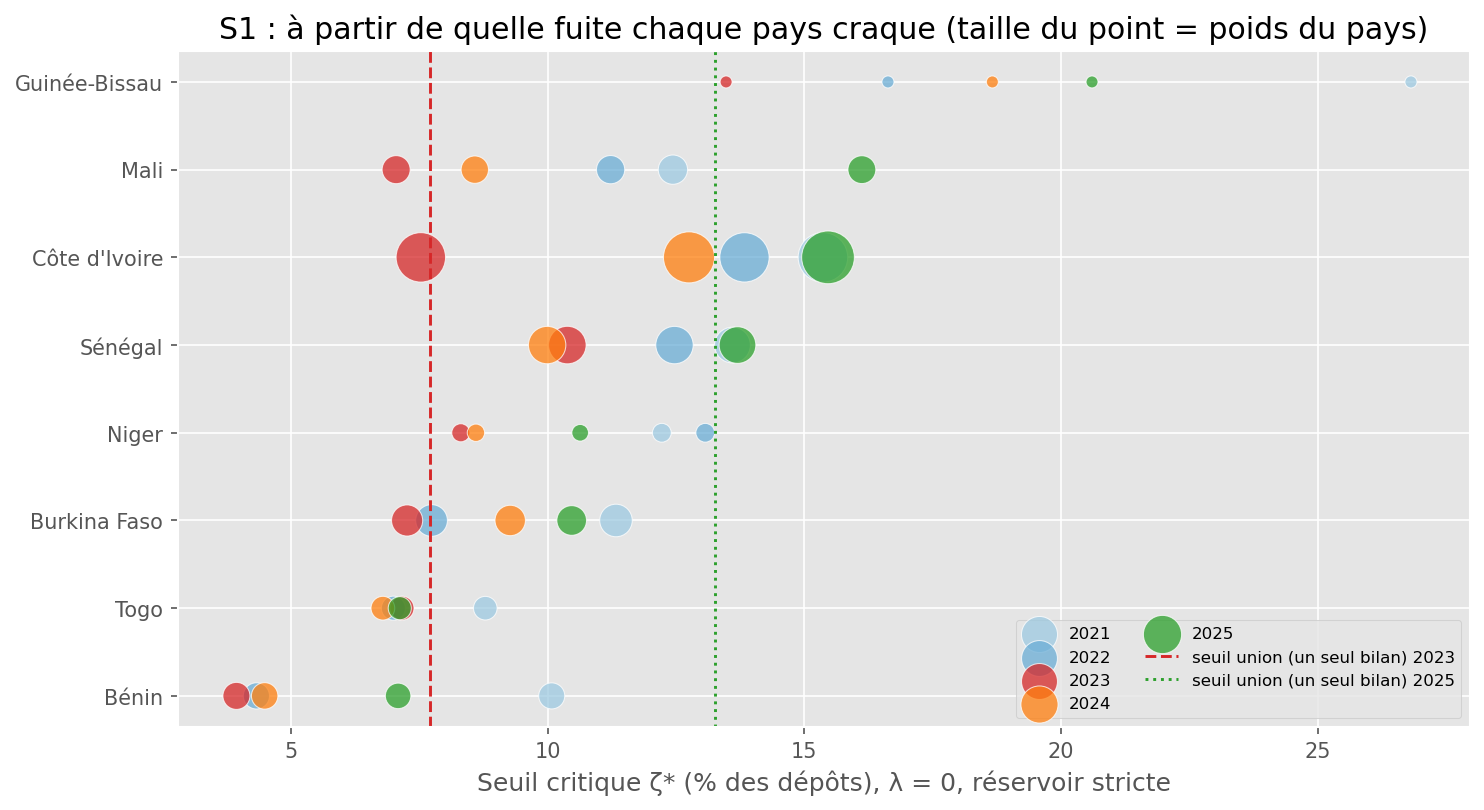
\includegraphics[width=1\textwidth]{S1_seuils_par_pays.png}
		\caption{Seuil critique de chaque pays, par année ($\lambda=0$, $b$ stricte). La taille du point est le poids du pays dans les dépôts de l'union.}\label{fig:seuils}
	\end{figure}
	
	\vspace{0.9cm}
	
	En montants, le seuil de l'union représente de 3\,463 milliards de FCFA (2023) à 7\,454 (2025), soit environ 3,1 à 3,9 fois l'encours de monnaie électronique de l'union à la même date. Cette comparaison n'a valeur que d'ordre de grandeur, puisque ces fonds ne sont pas des dépôts convertis. La réponse à Q1 est donc conditionnelle : sans aide de la BCEAO, les banques absorbent seules une fuite d'environ 4 à 13\,\% des dépôts selon le pays et l'année ; une fuite plus faible n'a aucun effet sur le crédit.
	
	\subsection{Courbes de contraction}
	
	La figure~\ref{fig:courbes} montre, pour 2023 (année de liquidité rare) et 2025 (année confortable), la baisse du crédit selon la fuite. La courbe est plate jusqu'au seuil, puis croissante. La différence entre la courbe bleue (un seul bilan) et la rouge (huit pays séparés) est le coût d'ignorer l'hétérogénéité.
	
	\begin{figure}[htbp]
		\centering
		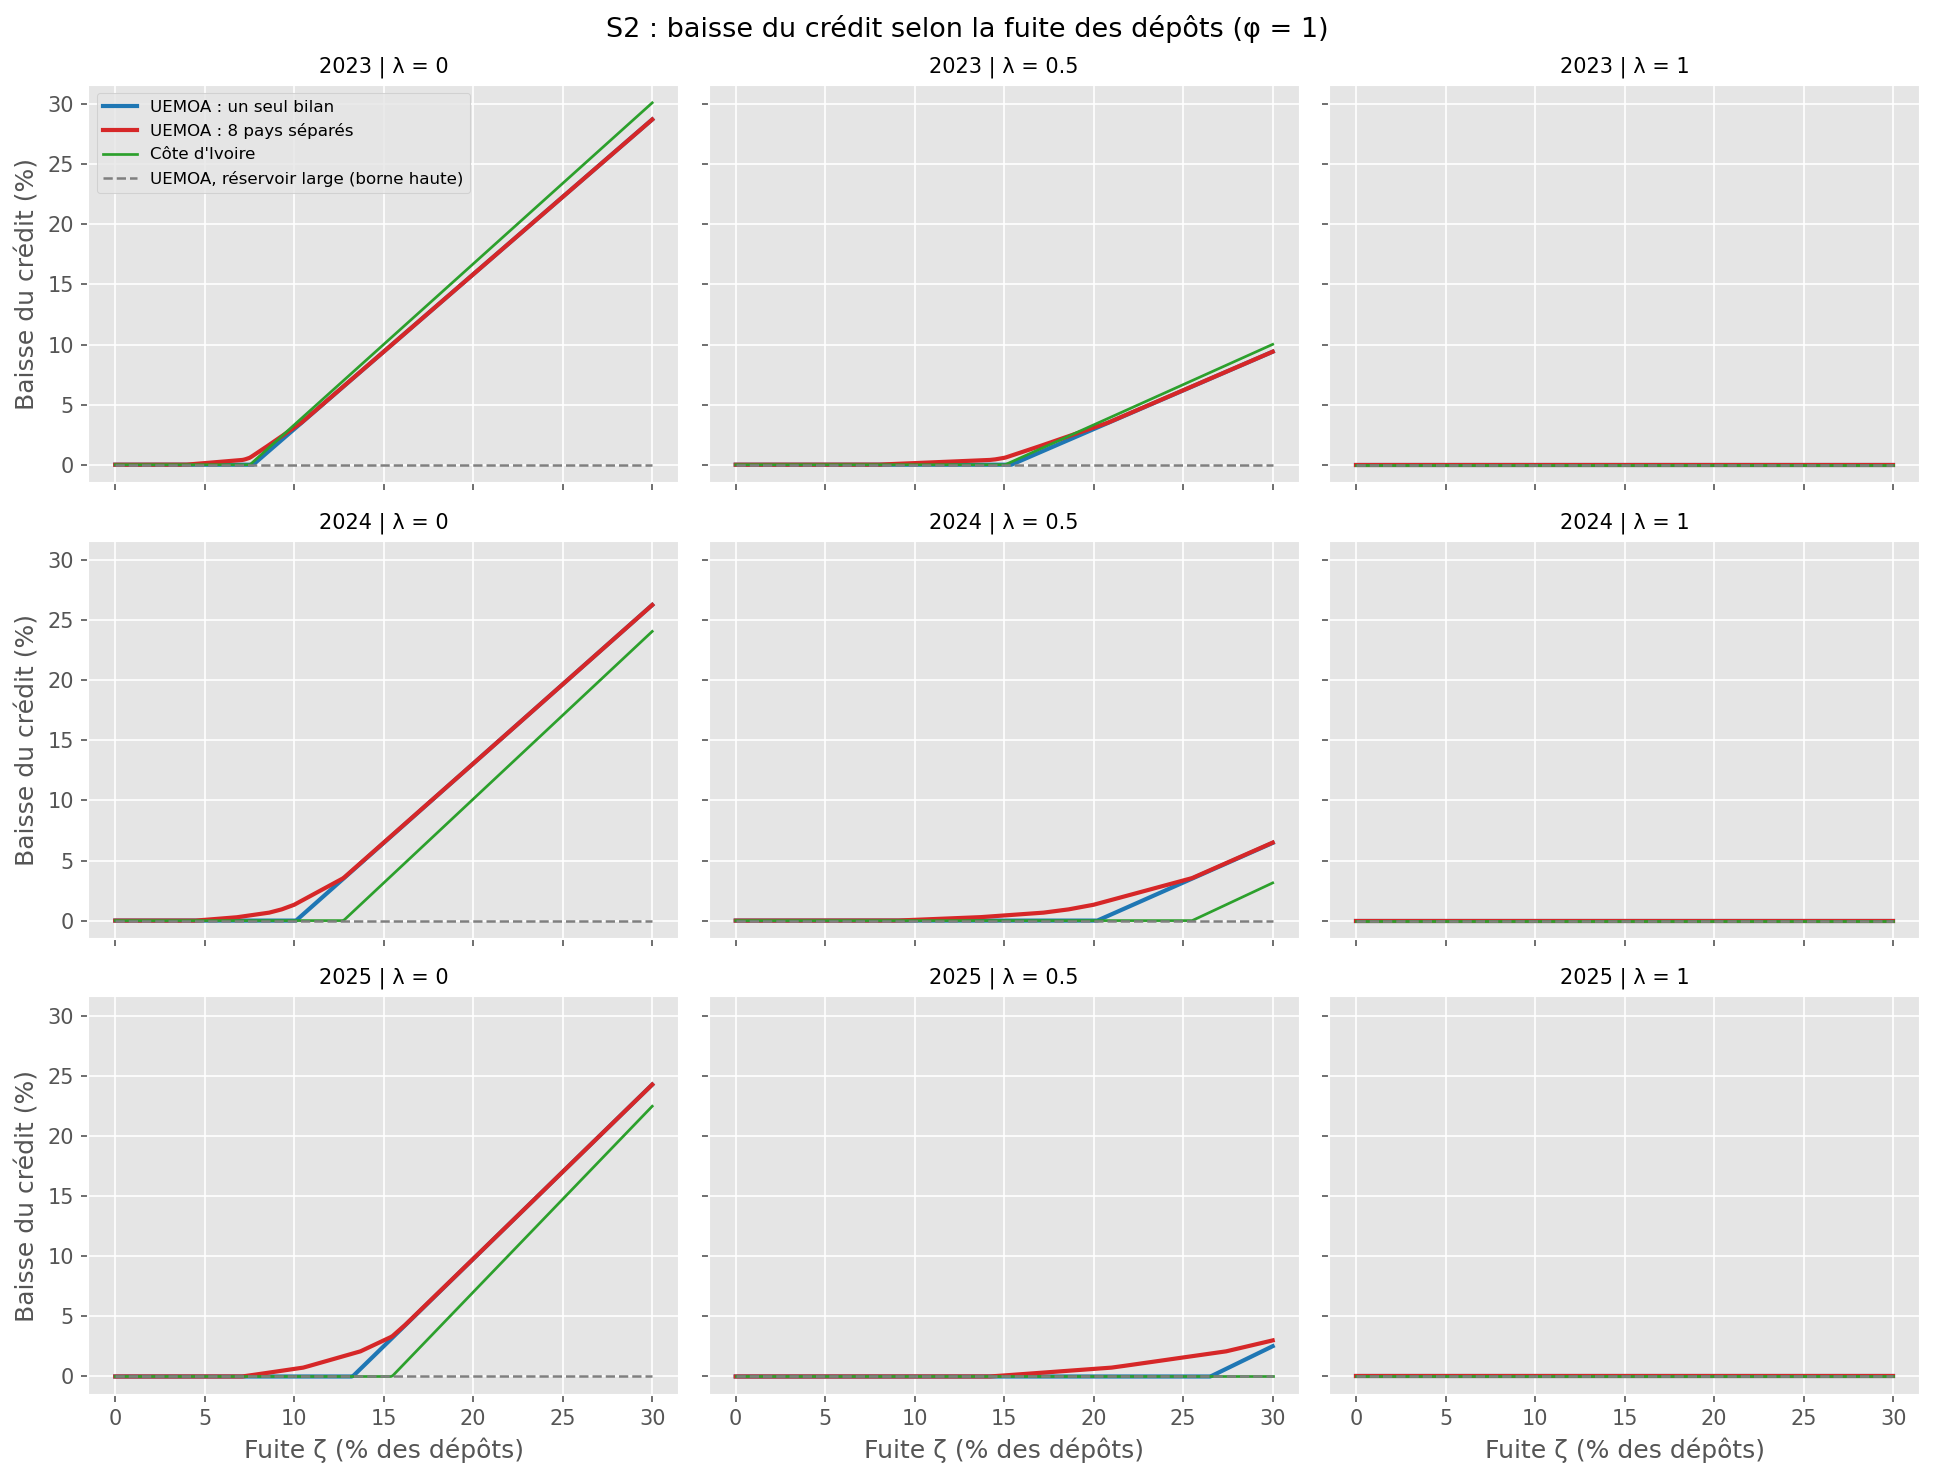
\includegraphics[width=1\textwidth]{S2_courbes_contraction.png}
		\caption{Baisse du crédit selon la fuite des dépôts ($\varphi=1$, $b$ stricte). Lignes : 2023 et 2025 ; colonnes : $\lambda=0$ et $\lambda=0{,}5$.}\label{fig:courbes}
	\end{figure}
	
	
	Le tableau~\ref{tab:cles} donne les chiffres-clés sur 2021--2025. À $\lambda=0$ et 10\,\% de fuite, le crédit de l'union baisse de 0\,\% à 3,0\,\% selon l'année en un seul bilan, de 0,1\,\% à 3,1\,\% pays par pays (de 33 à 1\,078 milliards de FCFA). À 15\,\%, de 2,5\,\% à 9,4\,\% ; à 20\,\%, de 9,7\,\% à 15,8\,\%.
	
	\begin{table}[htbp]
		\centering
		\caption{Baisse du crédit de l'union selon la fuite, fourchette sur 2021--2025 ($\varphi=1$, $b$ stricte)}\label{tab:cles}
		\small
		\begin{tabular}{llcccc}
			\toprule
			$\lambda$ & Fuite $\zeta$ & Un seul bilan (\%) & 8 pays séparés (\%) & 8 pays (Md FCFA) & Pays touchés \\
			\midrule
			0 & 5\,\%  & 0,0 & 0,0 -- 0,1 & 0 -- 46 & 0 -- 1 \\
			0 & 10\,\% & 0,0 -- 3,0 & 0,1 -- 3,1 & 33 -- 1\,078 & 1 -- 6 \\
			0 & 15\,\% & 2,5 -- 9,4 & 2,9 -- 9,4 & 796 -- 3\,285 & 5 -- 8 \\
			0 & 20\,\% & 9,7 -- 15,8 & 9,8 -- 15,8 & 2\,680 -- 5\,534 & 7 -- 8 \\
			\midrule
			0,5 & 10\,\% & 0,0 & 0,0 -- 0,1 & 0 -- 46 & 0 -- 1 \\
			0,5 & 15\,\% & 0,0 & 0,0 -- 0,6 & 0 -- 200 & 0 -- 4 \\
			0,5 & 20\,\% & 0,0 -- 3,0 & 0,1 -- 3,1 & 33 -- 1\,078 & 1 -- 6 \\
			0,5 & 30\,\% & 2,5 -- 9,4 & 2,9 -- 9,4 & 796 -- 3\,285 & 5 -- 8 \\
			\bottomrule
		\end{tabular}
	\end{table}
	
	\subsection{Hétérogénéité entre pays (Q3)}
	
	La figure~\ref{fig:carte} détaille, pays par pays, la baisse du crédit en pourcentage du crédit du pays. En 2023, une fuite de 10\,\% touche six pays : Bénin ($-8{,}5$\,\%, soit 261 milliards), Togo ($-4{,}2$\,\%), Mali ($-3{,}5$\,\%), Burkina Faso ($-3{,}4$\,\%), Côte d'Ivoire ($-3{,}3$\,\%, soit 399 milliards) et Niger ($-2{,}0$\,\%) ; ils concentrent 80\,\% des dépôts de l'union. En 2025, la même fuite ne touche que le Bénin ($-3{,}7$\,\%, 136 milliards) et le Togo ($-4{,}4$\,\%, 106 milliards), soit 15\,\% des dépôts, alors que le modèle agrégé n'indique aucune baisse. L'écart (0 contre 242 milliards, soit 0,6\,\% du crédit de l'union) est modeste en valeur relative mais concentré sur deux pays.
	
	\begin{figure}[htbp]
		\centering
		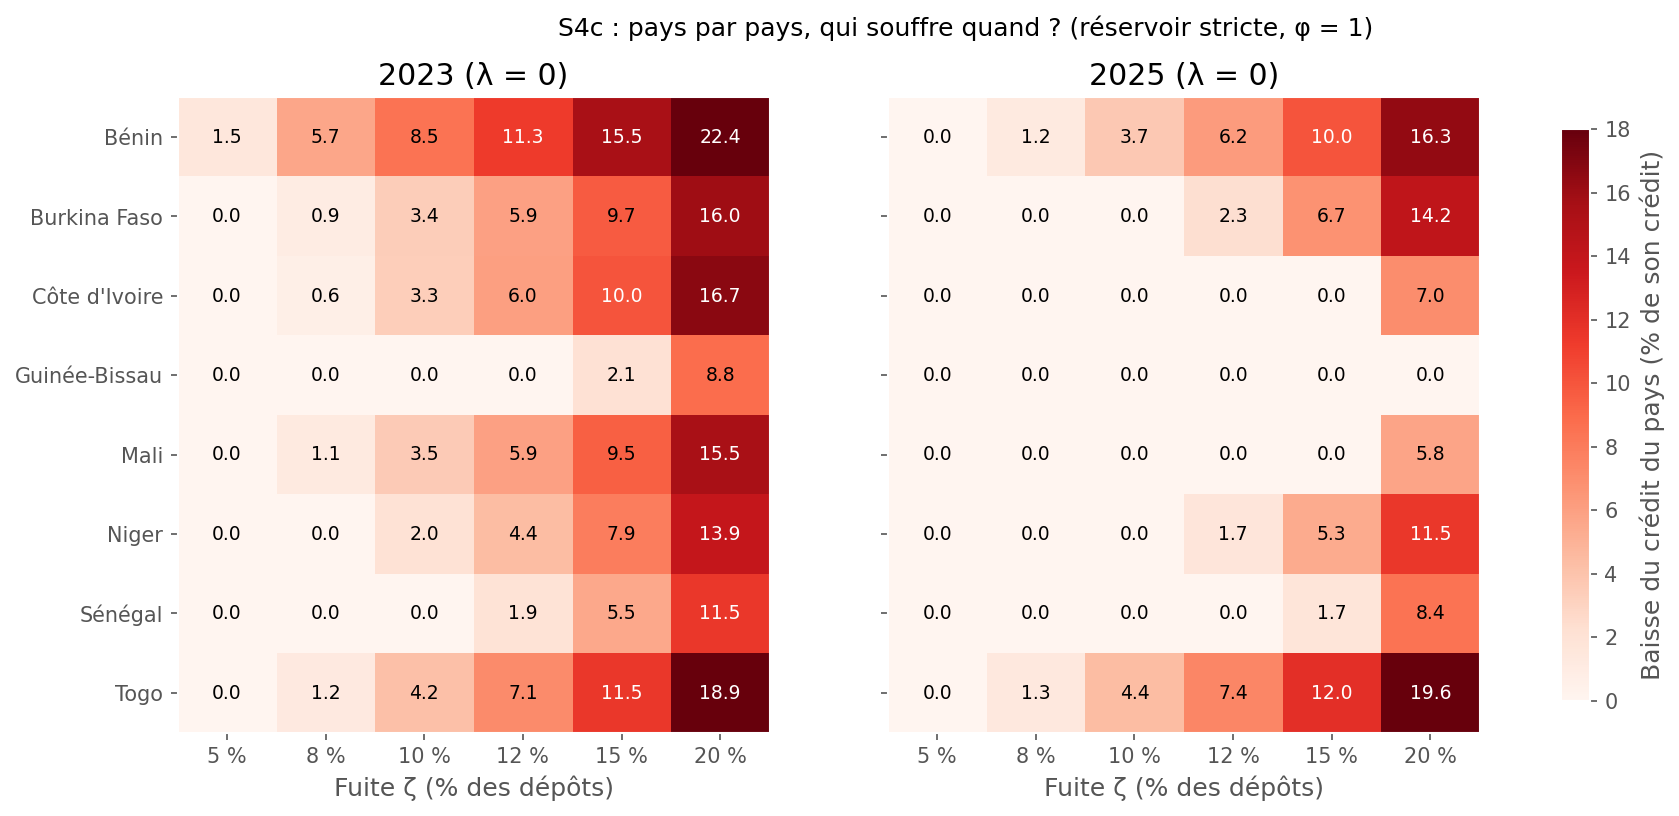
\includegraphics[width=1\textwidth]{S4c_carte_pays_fuite.png}
		\caption{Baisse du crédit de chaque pays (\% de son crédit) selon la fuite, 2023 et 2025 ($\lambda=0$, $\varphi=1$).}\label{fig:carte}
	\end{figure}
	
	Cette hétérogénéité compte surtout dans la zone intermédiaire : au-delà de 15\,\% de fuite, les courbes agrégée et par pays se confondent (figure~\ref{fig:courbes}). La part des dépôts de l'union située dans des pays au-delà de leur seuil est de 76\,\% en 2023 à 8\,\% de fuite, contre 15\,\% en 2025. Le modèle agrégé sous-estime donc la contraction (proposition~\ref{prop:jensen}), mais c'est la répartition de la charge entre pays qu'il masque le plus.
	
	\subsection{Le rôle du recyclage (Q2)}
	
	Le paramètre $\lambda$ décale le coude vers la droite (figure~\ref{fig:lambda}). Comme $\lambda$ n'intervient que par le produit $(1-\lambda)\zeta$, un recyclage de 50\,\% donne exactement le résultat d'une fuite deux fois plus petite : le seuil de l'union passe de 7,7--13,3\,\% à 15,4--26,5\,\%, et celui du pays le plus fragile de 3,9--8,8\,\% à 7,9--17,6\,\%. À $\lambda=1$, la contraction est nulle partout.
	
	\begin{figure}[htbp]
		\centering
		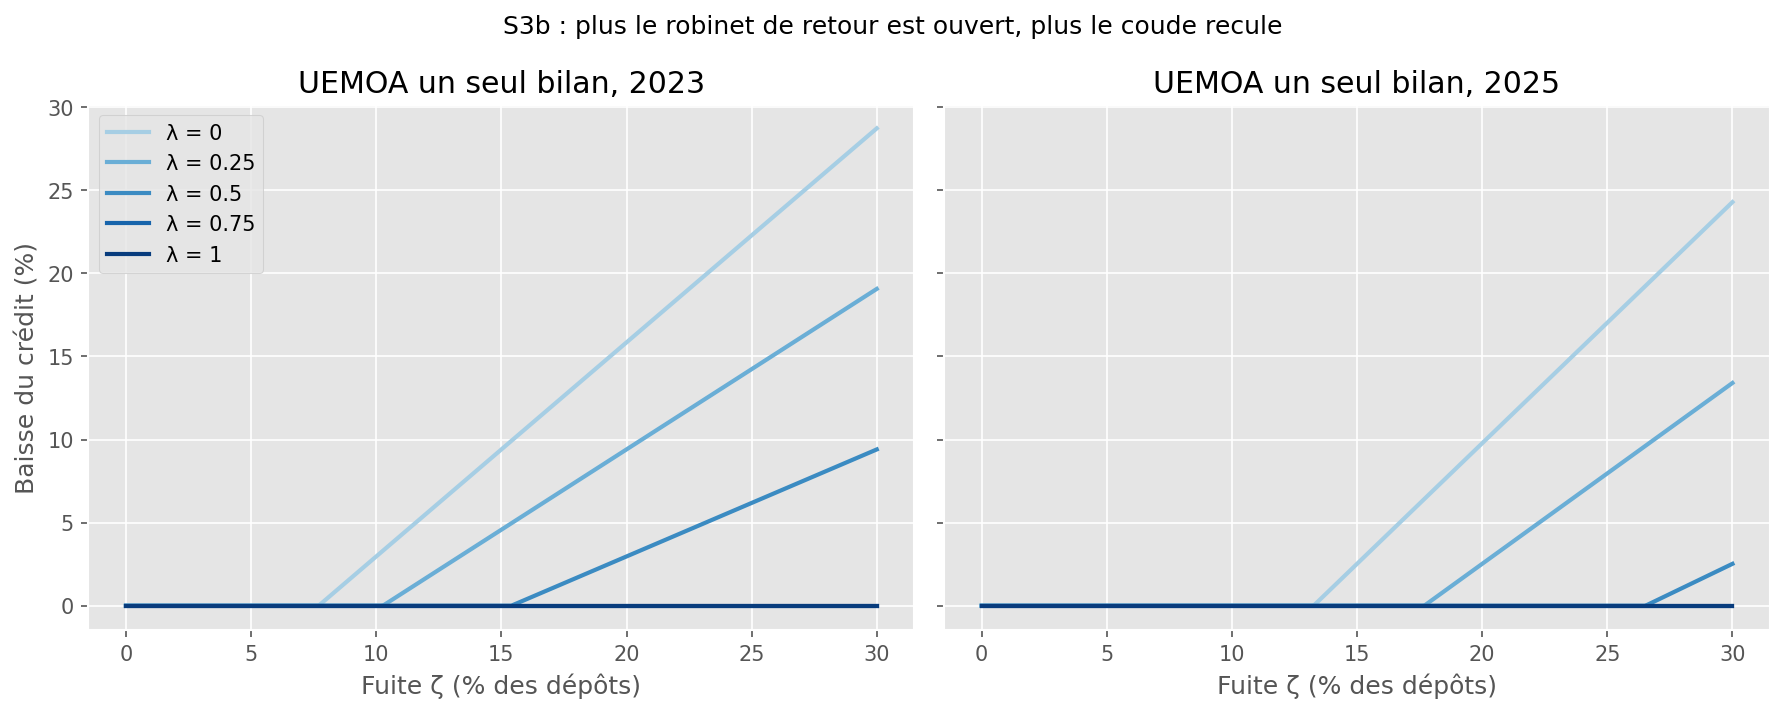
\includegraphics[width=1\textwidth]{S3b_effet_lambda.png}
		\caption{Baisse du crédit de l'union (un seul bilan) selon $\lambda$, 2023 et 2025 ($\varphi=1$, $b$ stricte).}\label{fig:lambda}
	\end{figure}
	
	Ce résultat est mécanique, mais il a une portée de politique : le levier le plus puissant n'est pas dans les bilans des banques, il est dans les mains de la BCEAO. Une banque centrale qui s'engagerait à refinancer les banques, contre collatéral éligible, neutraliserait le canal. À l'inverse, $\lambda=0$ est un cas de stress, non un cas central (hypothèse H3).
	
	\subsection{Plafond de détention}
	
	La figure~\ref{fig:plafond} applique la règle de la section~\ref{sec:cadre}. À $\lambda=0$, un plafond de 2\,\% des dépôts n'expose aucun pays, quelle que soit l'année. Un plafond de 5\,\% n'expose aucun pays en 2021 et en 2025, mais expose certains pays en 2022--2024. Un plafond de 10\,\% expose au moins un pays chaque année, et l'union entière en 2023. Un plafond de 20\,\% expose l'union entière chaque année. Avec $\lambda=0{,}5$, un plafond de 5\,\% n'expose personne, un plafond de 10\,\% expose certains pays en 2022--2024, et un plafond de 20\,\% l'union en 2023 seulement.
	
	\begin{figure}[htbp]
		\centering
		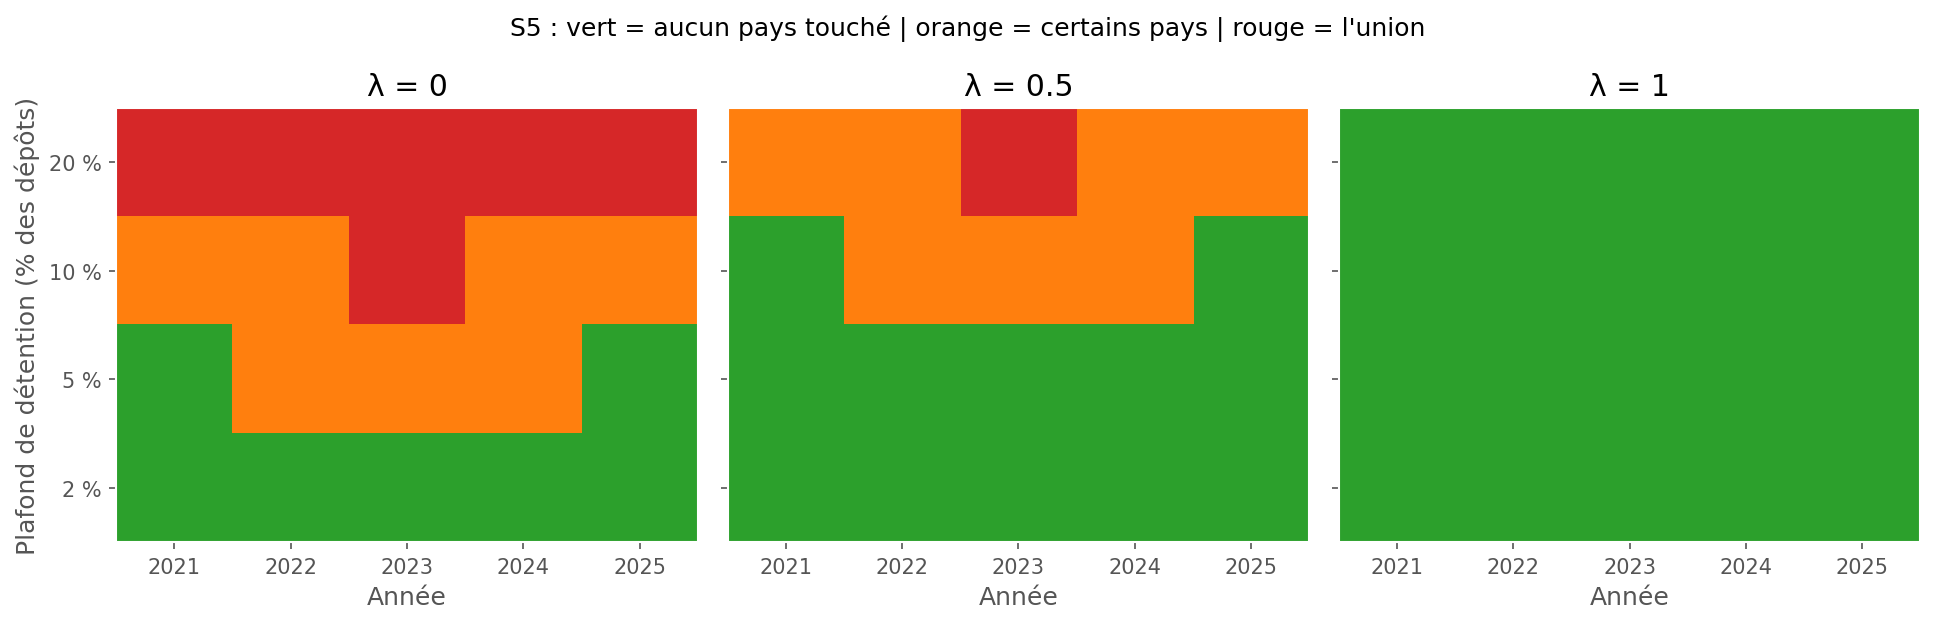
\includegraphics[width=1\textwidth]{S5_regle_plafond.png}
		\caption{Diagnostic du plafond de détention ($b$ stricte, $\varphi=1$). Vert : aucun pays touché ; orange : certains pays touchés ; rouge : l'union touchée.}\label{fig:plafond}
	\end{figure}
	
	Ces plafonds sont exprimés en part des dépôts. Pour les relier à un plafond individuel en francs CFA, il faudrait connaître le nombre d'utilisateurs éligibles et leur plafond, ce qui n'est pas possible aujourd'hui. À titre de comparaison, \citet{meller2023} estiment qu'un plafond de 3\,000 euros correspond à environ 15\,\% des dépôts de détail de la zone euro.
	
	\subsection{Zoom sur la Côte d'Ivoire}
	
	La Côte d'Ivoire pèse 41\,\% des dépôts de l'union en 2025. À $\lambda=0$, une fuite de 10\,\% réduit son crédit de 3,3\,\% (399 milliards) en 2023 et de 0\,\% les autres années ; à 15\,\%, de 0\,\% à 10,0\,\% (jusqu'à 1\,204 milliards) ; à 20\,\%, de 6,7\,\% à 16,7\,\% (650 à 2\,010 milliards). Comme les dépôts à vue représentent 64,7\,\% de $D$, si seuls ceux-ci migrent, une fuite de 10\,\% de l'ensemble des dépôts équivaut à environ 15\,\% des dépôts à vue.
	
	\begin{figure}[htbp]
		\centering
		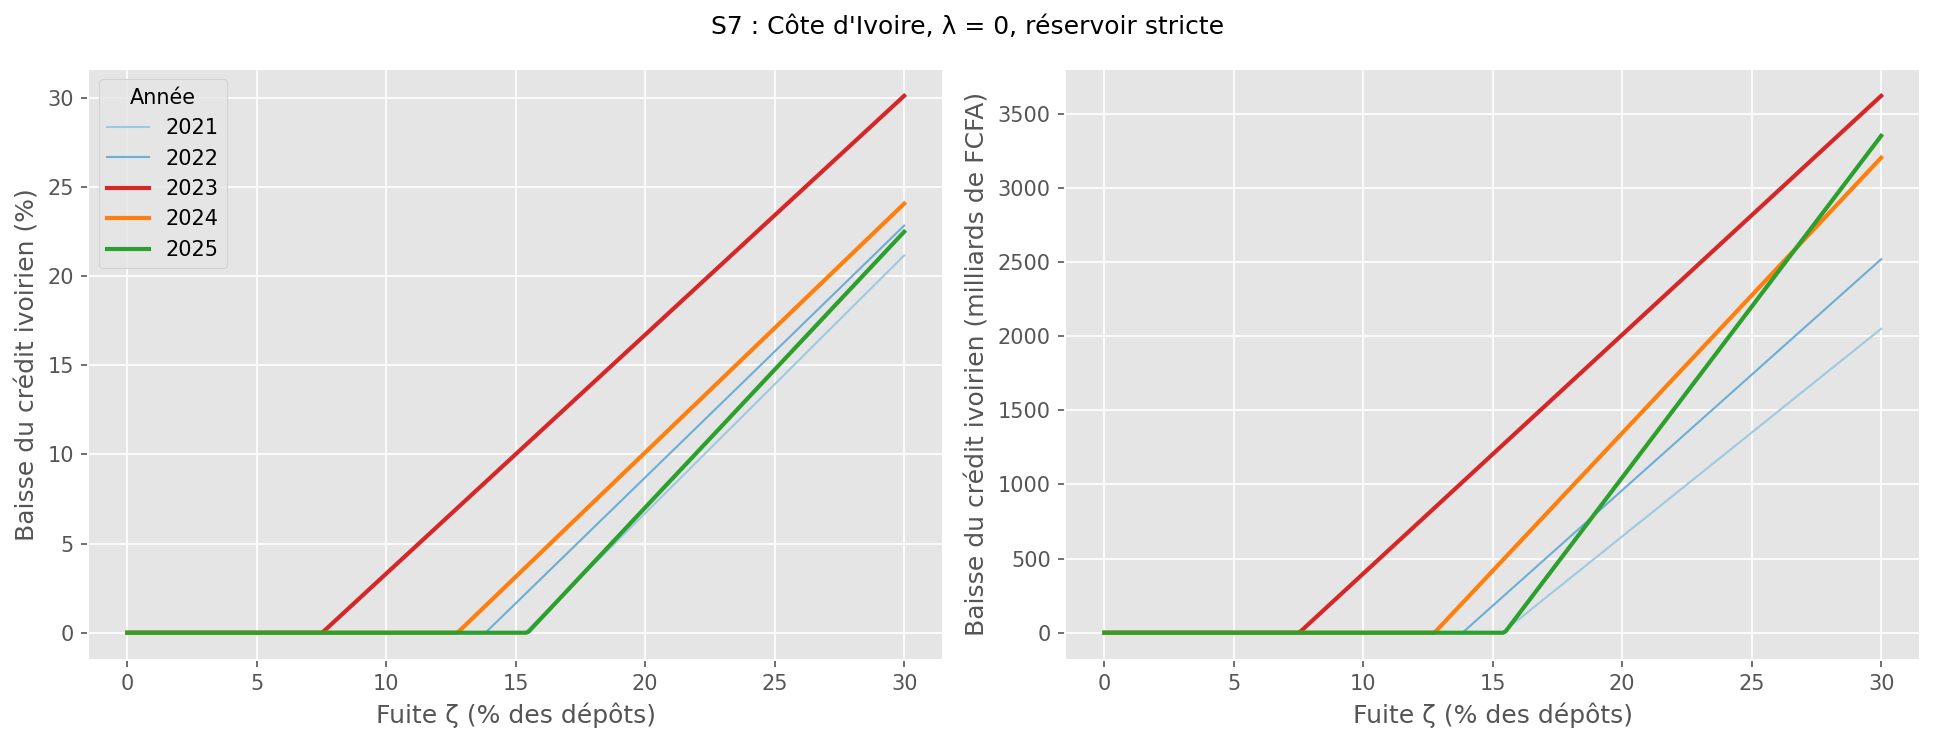
\includegraphics[width=1\textwidth]{S7_zoom_cote_ivoire.png}
		\caption{Côte d'Ivoire : baisse du crédit en \% et en milliards de FCFA ($\lambda=0$, $b$ stricte, $\varphi=1$).}\label{fig:ci}
	\end{figure}
	
	\subsection{Robustesse}
	
	\paragraph{Répercussion $\varphi$.}\label{sec:phi} Le seuil ne dépend pas de $\varphi$ ; seule la pente change. Le tableau~\ref{tab:phi} montre la baisse du crédit pour $\varphi\in\{0{,}25;0{,}5;1\}$. Avec $\varphi=0{,}25$, la contraction de l'union pays par pays en 2023 à 10\,\% de fuite est de 0,8\,\% (269 milliards) au lieu de 3,1\,\% (1\,078 milliards).
	
	\begin{table}[htbp]
		\centering
		\caption{Baisse du crédit de l'union (8 pays séparés) selon $\varphi$, $\lambda=0$}\label{tab:phi}
		\small
		\begin{tabular}{llccc}
			\toprule
			Année & Fuite $\zeta$ & $\varphi=0{,}25$ & $\varphi=0{,}5$ & $\varphi=1$ \\
			\midrule
			2023 & 10\,\% & 0,8\,\% (269 Md) & 1,5\,\% (539 Md) & 3,1\,\% (1\,078 Md) \\
			2023 & 15\,\% & 2,4\,\% (821 Md) & 4,7\,\% (1\,642 Md) & 9,4\,\% (3\,285 Md) \\
			2023 & 20\,\% & 4,0\,\% (1\,383 Md) & 7,9\,\% (2\,767 Md) & 15,8\,\% (5\,534 Md) \\
			2025 & 10\,\% & 0,2\,\% (61 Md) & 0,3\,\% (121 Md) & 0,6\,\% (242 Md) \\
			2025 & 15\,\% & 0,8\,\% (291 Md) & 1,5\,\% (582 Md) & 3,0\,\% (1\,163 Md) \\
			2025 & 20\,\% & 2,4\,\% (947 Md) & 4,9\,\% (1\,894 Md) & 9,8\,\% (3\,788 Md) \\
			\bottomrule
		\end{tabular}
	\end{table}
	
	\paragraph{Erreur de mesure du matelas $\kappa$.}\label{sec:kappa} La figure~\ref{fig:kappa} montre comment les seuils bougent si le vrai matelas est $\kappa b$. Pour $\kappa=0{,}5$, le seuil de l'union devient 3,8 à 6,6\,\% (au lieu de 7,7 à 13,3\,\%) et celui du pays le plus fragile 2,0 à 4,4\,\%. Pour $\kappa=1{,}25$, ils montent de 25\,\%. Le plafond de 2\,\% résiste à une surestimation du matelas de 49\,\% (2023) à 77\,\% (2021) ; un plafond de 5\,\% ne protège plus en 2022--2024 avec la mesure actuelle, et un plafond de 10\,\% ne protège dans aucune année.
	
	\begin{figure}[htbp]
		\centering
		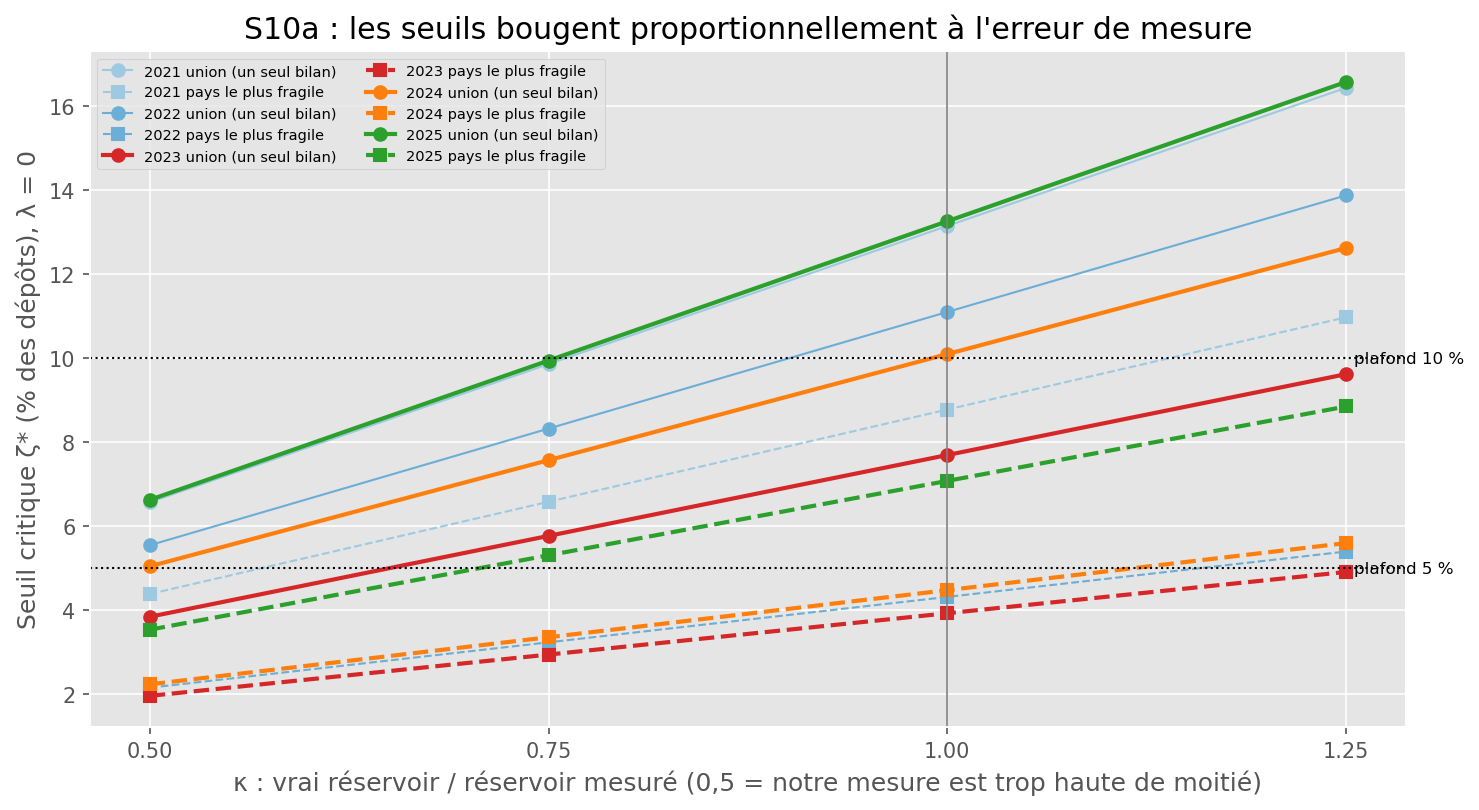
\includegraphics[width=1\textwidth]{S10a_seuils_selon_kappa.png}
		\caption{Seuils selon l'erreur de mesure du matelas ($\lambda=0$). Trait plein : union ; pointillés : pays le plus fragile.}\label{fig:kappa}
	\end{figure}
	
	La conclusion « les banques absorbent jusqu'à environ 4 à 13\,\% » est donc sensible à la mesure de $b$ ; la règle la plus robuste est celle du plafond de 2\,\%.
	
	\newpage
	
	% =============================================================================
	\section{Discussion et limites}\label{sec:discussion}
	% =============================================================================
	
	\paragraph{Ce que les résultats permettent d'affirmer.} Sous l'hypothèse d'une migration progressive de dépôts, sans aide de la BCEAO, la liquidité actuelle des banques en monnaie de banque centrale absorberait une conversion de 4 à 9\,\% des dépôts avant qu'un pays ne réduise son crédit, et de 8 à 13\,\% pour l'union vue comme un seul bilan, selon l'année. Au-delà, la contraction dépend surtout de deux choix de politique : le recyclage (refinancement de la BCEAO) et le plafond de détention.
	
	\paragraph{Comparaison avec la zone euro.} Nos seuils (7,7 à 13,3\,\% pour l'union) sont plus bas que les capacités d'absorption de la zone euro rapportées par \citet{meller2023} (de 12\,\% à 20\,\% selon les années et les hypothèses). Il ne faut pas en conclure que l'UEMOA est plus fragile : leur dénominateur est les dépôts de détail à vue, leur numérateur inclut les billets, et ils appliquent des contraintes de ratio de liquidité absentes de l'union. Les ordres de grandeur ne se comparent que prudemment.
	
	\paragraph{Limites principales.}
	\begin{enumerate}[nosep,label=(\roman*)]
		\item \emph{Borne haute sur le crédit.} Le rationnement des quantités ($\varphi=1$) est plus brutal que le mécanisme de second tour de la littérature \citep{kumhof2018, bouis2024}. Les résultats pour $\varphi<1$ sont plus faibles dans la même proportion (tableau~\ref{tab:phi}). Inversement, l'absence de rétroaction du crédit sur les dépôts (H4) sous-estime la contraction.
		\item \emph{La fuite n'est pas forcément une fuite de dépôts.} Dans une économie où l'espèce domine, une MNBC peut d'abord puiser dans les billets \citep{bouis2024}, et le mobile money apparaît complémentaire aux dépôts \citep{trinnou2023}. Le paramètre $\pi$ (section~\ref{sec:incertitude}) n'est pas estimé ici ; les seuils exprimés en émission totale de MNBC seraient plus élevés.
		\item \emph{Pas de ruée.} Une panique bancaire \citep{diamond1983} déplacerait des montants bien supérieurs en peu de temps ; \citet{schilling2024} et \citet{bidder2024} montrent que sa probabilité dépend du design. L'absence d'effet à fuite modérée ne vaut que pour une migration progressive.
		\item \emph{Mesure du matelas.} Les comptes ordinaires débiteurs incluent des avoirs étrangers et interbancaires ; les réserves obligatoires sont approximées ; les chiffres de 2025 sont provisoires. Le test sur $\kappa$ en borne l'effet mais ne le supprime pas.
		\item \emph{Hétérogénéité sous-estimée.} Les données par pays ne montrent pas la dispersion entre banques d'un même pays, que l'on sait importante \citep{adalid2022, fritz2024}. Les seuils des banques les plus fragiles sont plus bas que ceux des pays.
		\item \emph{Paramètres communs.} $\zeta$ et $\lambda$ sont supposés identiques dans les huit pays alors que la bancarisation et l'accès au refinancement diffèrent.
		\item \emph{Absence de dynamique et de linéarité réaliste.} La pente au-delà du seuil n'est pas un résultat : elle découle de la forme retenue. Une dispersion des matelas entre banques, une décote sur les titres vendus ou un ajustement par les taux arrondiraient le coude.
	\end{enumerate}
	
	\paragraph{Implications de politique économique.} Sous ces réserves, trois messages ressortent. D'abord, un engagement de refinancement de la BCEAO neutralise le canal bancaire : c'est le levier le plus puissant. Ensuite, un plafond de détention bas protège tous les pays, y compris les plus fragiles ; sa valeur exacte dépend de la mesure du matelas. Enfin, la politique doit regarder le pays le plus fragile et non la moyenne de l'union, car les charges se concentrent sur quelques pays. Ces messages sont des conséquences du modèle, pas des recommandations fondées sur un coût-bénéfice complet.
	
	% =============================================================================
	\section{Conclusion}\label{sec:conclusion}
	% =============================================================================
	
	Cet article a posé, pour une MNBC qui n'existe pas dans l'UEMOA, une question conditionnelle : à quelles conditions une migration de dépôts devient-elle une contraction du crédit ? La réponse tient en un seuil, $\zs=b/(1-\lambda)$, que la calibration sur les bilans des huit pays situe entre 7,7 et 13,3\,\% des dépôts pour l'union et entre 3,9 et 8,8\,\% pour le pays le plus fragile, sans aide de la banque centrale. En deçà, le crédit ne bouge pas ; au-delà, il baisse, et l'effet dépend du recyclage et du plafond de détention plus que de la technologie.
	
	Ces conclusions sont conditionnelles à une mesure approximative de la liquidité, qui peut être surestimée, et à une migration progressive. Les prolongements les plus utiles sont l'introduction d'une dispersion des matelas entre banques, l'estimation de la part de la MNBC financée par des dépôts plutôt que par des espèces, un traitement des ruées, et l'actualisation avec les chiffres définitifs de 2025.
	

\newpage
	% =============================================================================
	\appendix
	\section{Démonstrations}\label{app:preuves}
	% =============================================================================
	
	\paragraph{Proposition~\ref{prop:seuil}.} Pour $\lambda<1$, $\Delta L_k>0$ si et seulement si $(1-\lambda)\zeta-b_k>0$, soit $\zeta>\zs_k$. Au-delà, $\Delta L_k/L_k=\varphi\big((1-\lambda)\zeta-b_k\big)/\rho_k$ est affine en $\zeta$, de pente $\varphi(1-\lambda)/\rho_k$. Pour $\lambda=1$, $(1-\lambda)\zeta-b_k=-b_k\le0$ : le déficit est nul.
	
	\paragraph{Proposition~\ref{prop:jensen}.} Par convexité de $x\mapsto\max\{0,x\}$ et inégalité de Jensen avec les poids $w_k$ : $\sum_k w_k\max\{0,x_k\}\ge\max\{0,\sum_k w_k x_k\}$. En multipliant par $\varphi D$, le membre de gauche est la contraction en valeur (en l'absence de plafonnement à $L_k$) pays par pays ; celui de droite est la contraction du modèle agrégé. Pour les seuils, $\bar b=\sum_k w_k b_k\ge\min_k b_k$, donc $\zs_{agg}\ge\zs_{\min}$.
	
	\paragraph{Proportionnalité au coefficient $\kappa$.} Si le matelas utilisable est $\kappa b_k$, le seuil du pays devient $\kappa b_k/(1-\lambda)=\kappa\,\zs_k$, de même pour $\zs_{\min}$ et $\zs_{agg}$.
	
	% =============================================================================
	\section{Données détaillées}\label{app:donnees}
	% =============================================================================
	
	\begin{table}[htbp]
		\centering
		\caption{Ratio crédit/dépôts $\rho_k$ par pays}\label{tab:rho}
		\small
		\begin{tabular}{lccccc}
			\toprule
			Pays & 2021 & 2022 & 2023 & 2024 & 2025 \\
			\midrule
			Bénin & 0,584 & 0,679 & 0,716 & 0,775 & 0,790 \\
			Burkina Faso & 0,674 & 0,776 & 0,799 & 0,768 & 0,674 \\
			Côte d'Ivoire & 0,692 & 0,708 & 0,746 & 0,717 & 0,647 \\
			Guinée-Bissau & 0,675 & 0,794 & 0,742 & 0,669 & 0,728 \\
			Mali & 0,728 & 0,827 & 0,838 & 0,808 & 0,674 \\
			Niger & 0,851 & 0,877 & 0,844 & 0,874 & 0,817 \\
			Sénégal & 0,814 & 0,787 & 0,836 & 0,804 & 0,747 \\
			Togo & 0,602 & 0,677 & 0,680 & 0,698 & 0,657 \\
			\bottomrule
		\end{tabular}
	\end{table}
	
	\begin{table}[htbp]
		\centering
		\caption{Seuils du modèle selon $\lambda$ (union et pays le plus fragile)}\label{tab:seuils-lambda}
		\small
		\begin{tabular}{lcccccc}
			\toprule
			& 2021 & 2022 & 2023 & 2024 & 2025 \\
			\midrule
			$\zs_{agg}$, $\lambda=0$ & 13,2\,\% & 11,1\,\% & 7,7\,\% & 10,1\,\% & 13,3\,\% \\
			$\zs_{\min}$, $\lambda=0$ & 8,8\,\% & 4,3\,\% & 3,9\,\% & 4,5\,\% & 7,1\,\% \\
			$\zs_{agg}$, $\lambda=0{,}5$ & 26,3\,\% & 22,2\,\% & 15,4\,\% & 20,2\,\% & 26,5\,\% \\
			$\zs_{\min}$, $\lambda=0{,}5$ & 17,6\,\% & 8,6\,\% & 7,9\,\% & 9,0\,\% & 14,2\,\% \\
			Seuil agrégé en Md FCFA, $\lambda=0$ & 5\,117 & 4\,858 & 3\,463 & 4\,892 & 7\,454 \\
			\bottomrule
		\end{tabular}
	\end{table}
	
	\begin{table}[htbp]
		\centering
		\caption{Seuils de l'union et du pays le plus fragile selon $\kappa$ ($\lambda=0$)}\label{tab:kappa}
		\small
		\begin{tabular}{lccccc}
			\toprule
			$\kappa$ & 2021 & 2022 & 2023 & 2024 & 2025 \\
			\midrule
			\multicolumn{6}{l}{\emph{Union (un seul bilan)}} \\
			0,5 & 6,6\,\% & 5,6\,\% & 3,8\,\% & 5,1\,\% & 6,6\,\% \\
			1 & 13,2\,\% & 11,1\,\% & 7,7\,\% & 10,1\,\% & 13,3\,\% \\
			1,25 & 16,4\,\% & 13,9\,\% & 9,6\,\% & 12,6\,\% & 16,6\,\% \\
			\multicolumn{6}{l}{\emph{Pays le plus fragile}} \\
			0,5 & 4,4\,\% & 2,2\,\% & 2,0\,\% & 2,2\,\% & 3,5\,\% \\
			1 & 8,8\,\% & 4,3\,\% & 3,9\,\% & 4,5\,\% & 7,1\,\% \\
			1,25 & 11,0\,\% & 5,4\,\% & 4,9\,\% & 5,6\,\% & 8,9\,\% \\
			\bottomrule
		\end{tabular}
	\end{table}
	
	% =============================================================================
	\section{Figures complémentaires}\label{app:figures}
	% =============================================================================
	
	\begin{figure}[htbp]
		\centering
		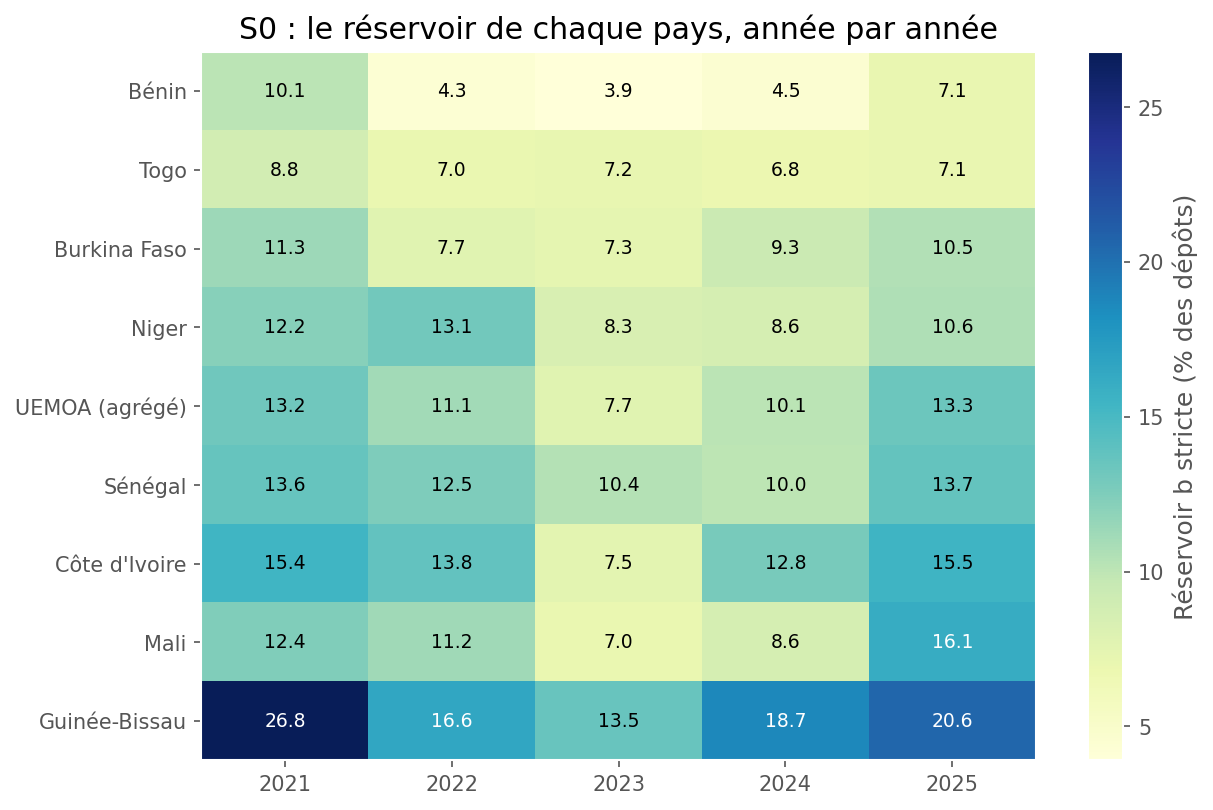
\includegraphics[width=1\textwidth]{S0_carte_reservoirs.png}
		\caption{Matelas $b$ de chaque pays et année (carte de chaleur).}
	\end{figure}
	
	\begin{figure}[htbp]
		\centering
		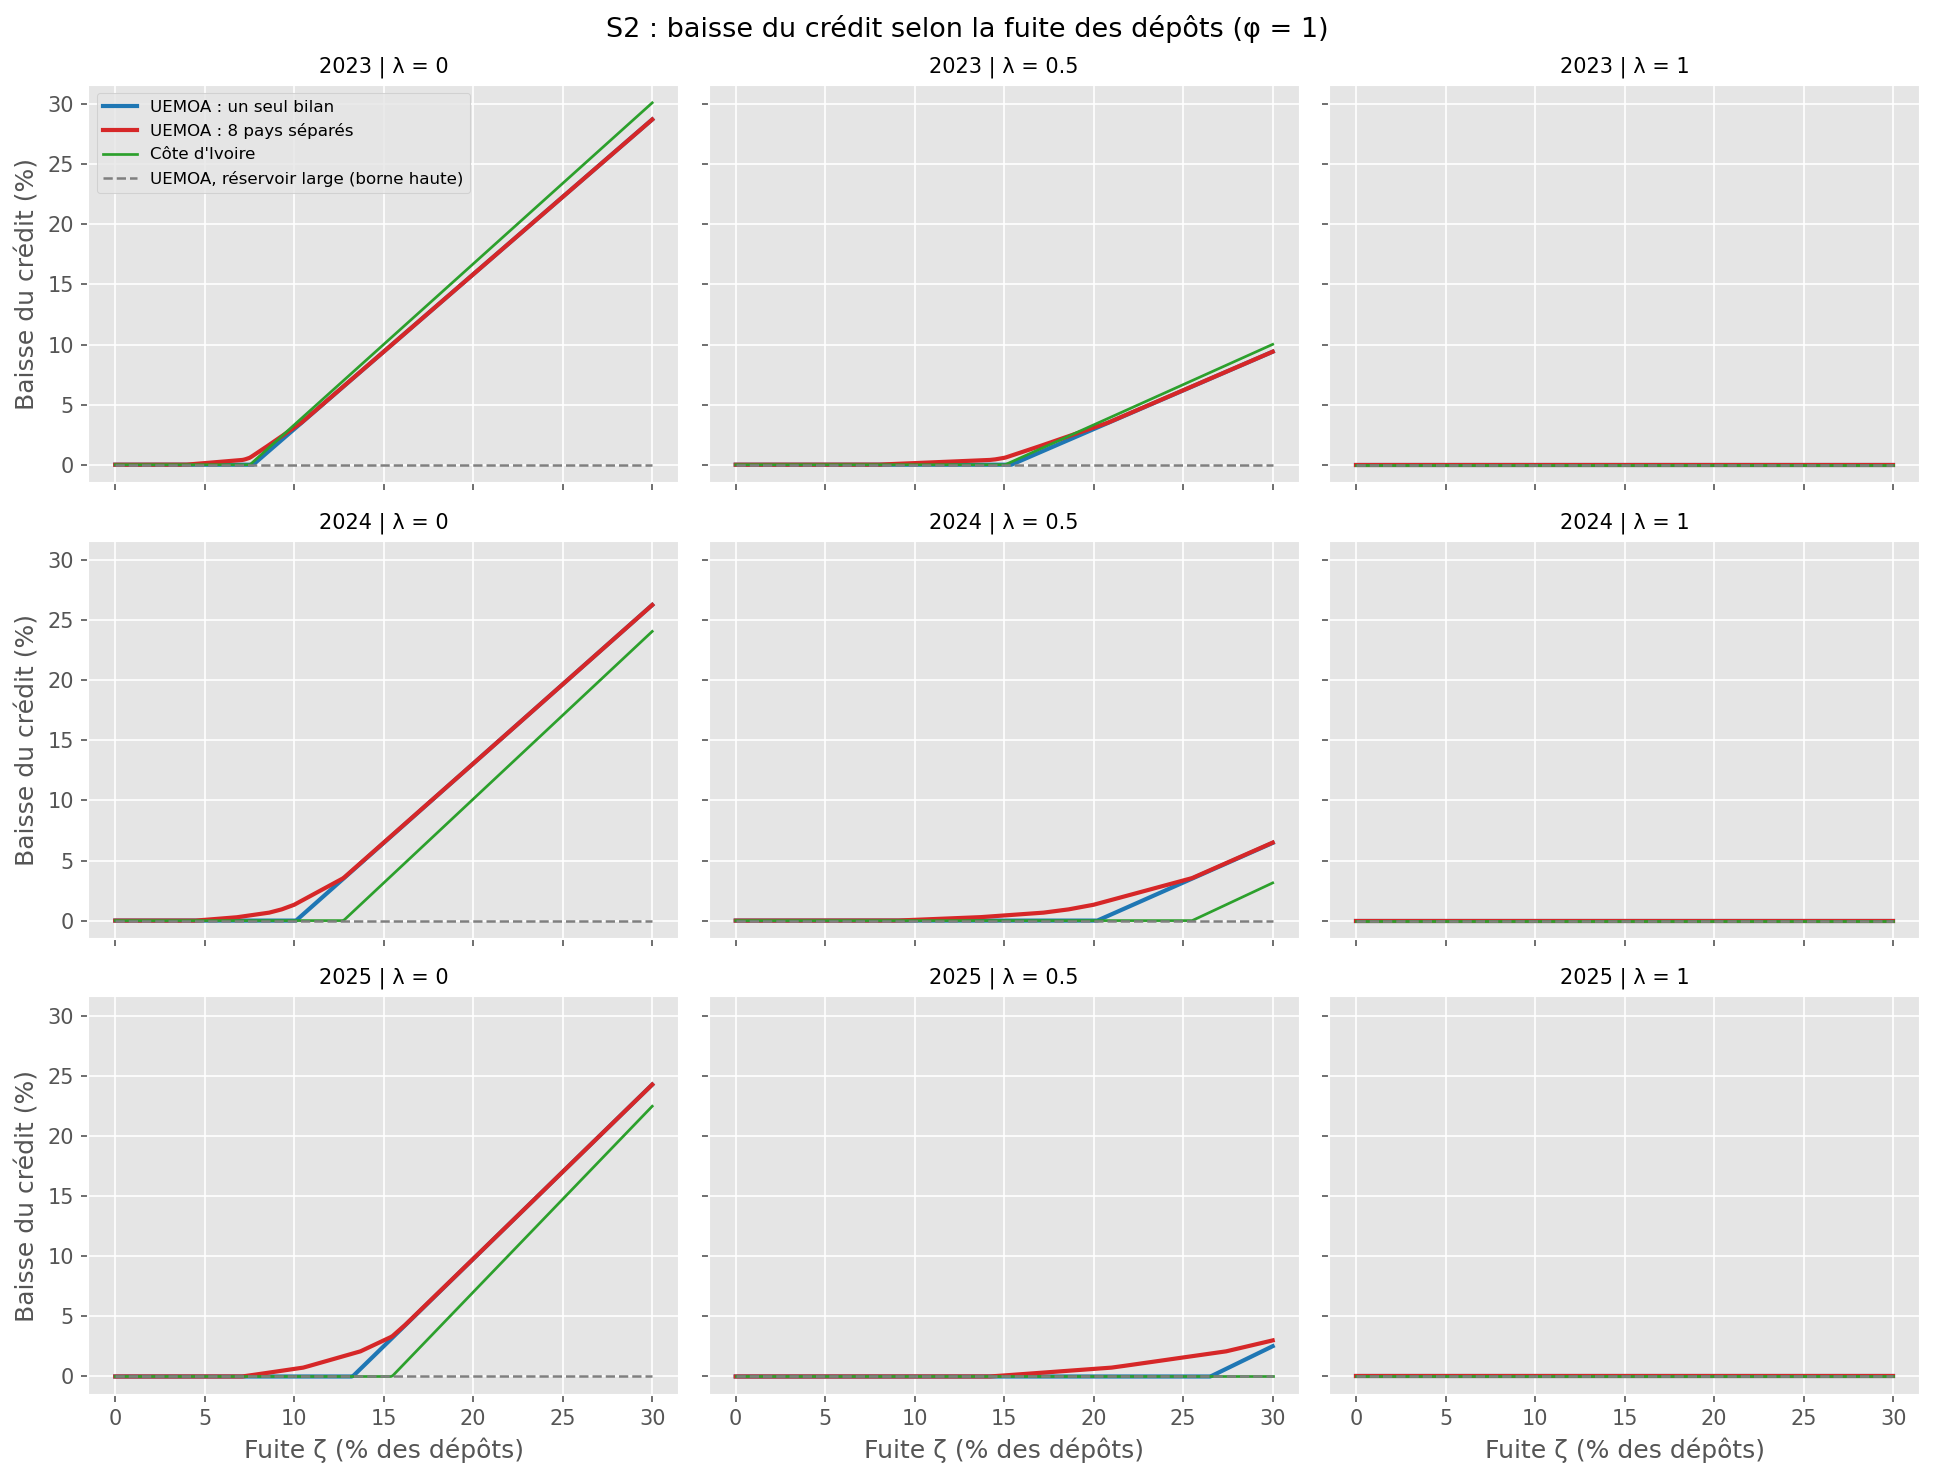
\includegraphics[width=1\textwidth]{S2_courbes_contraction.png}
		\caption{Baisse du crédit selon la fuite : version complète (2023, 2024, 2025 ; $\lambda\in\{0;0{,}5;1\}$) avec le matelas large en borne haute (pointillés).}
	\end{figure}
	
	\begin{figure}[htbp]
		\centering
		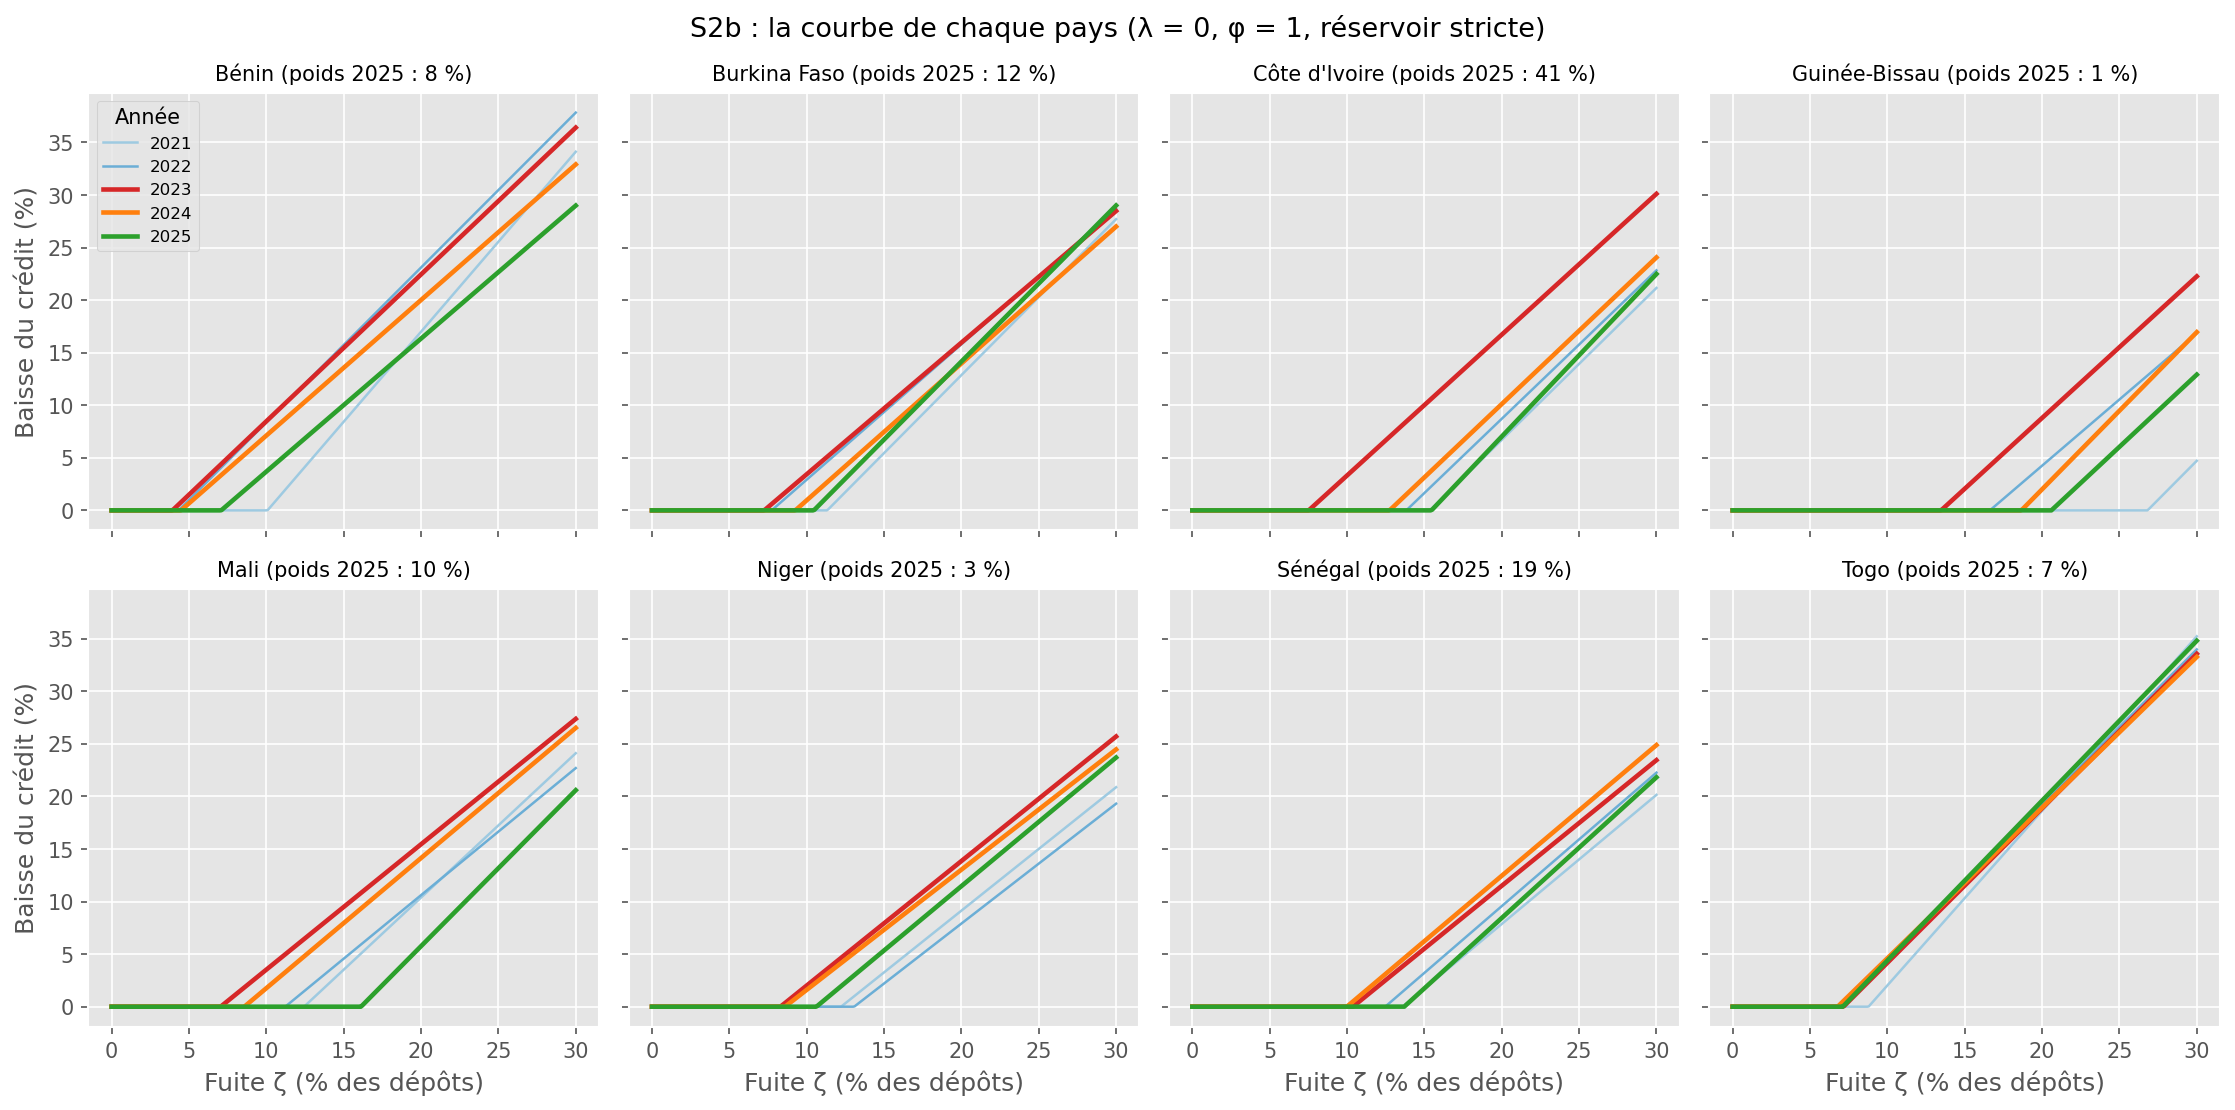
\includegraphics[width=1\textwidth]{S2b_courbes_par_pays.png}
		\caption{Courbe de contraction de chaque pays, par année ($\lambda=0$).}
	\end{figure}
	
	\begin{figure}[htbp]
		\centering
		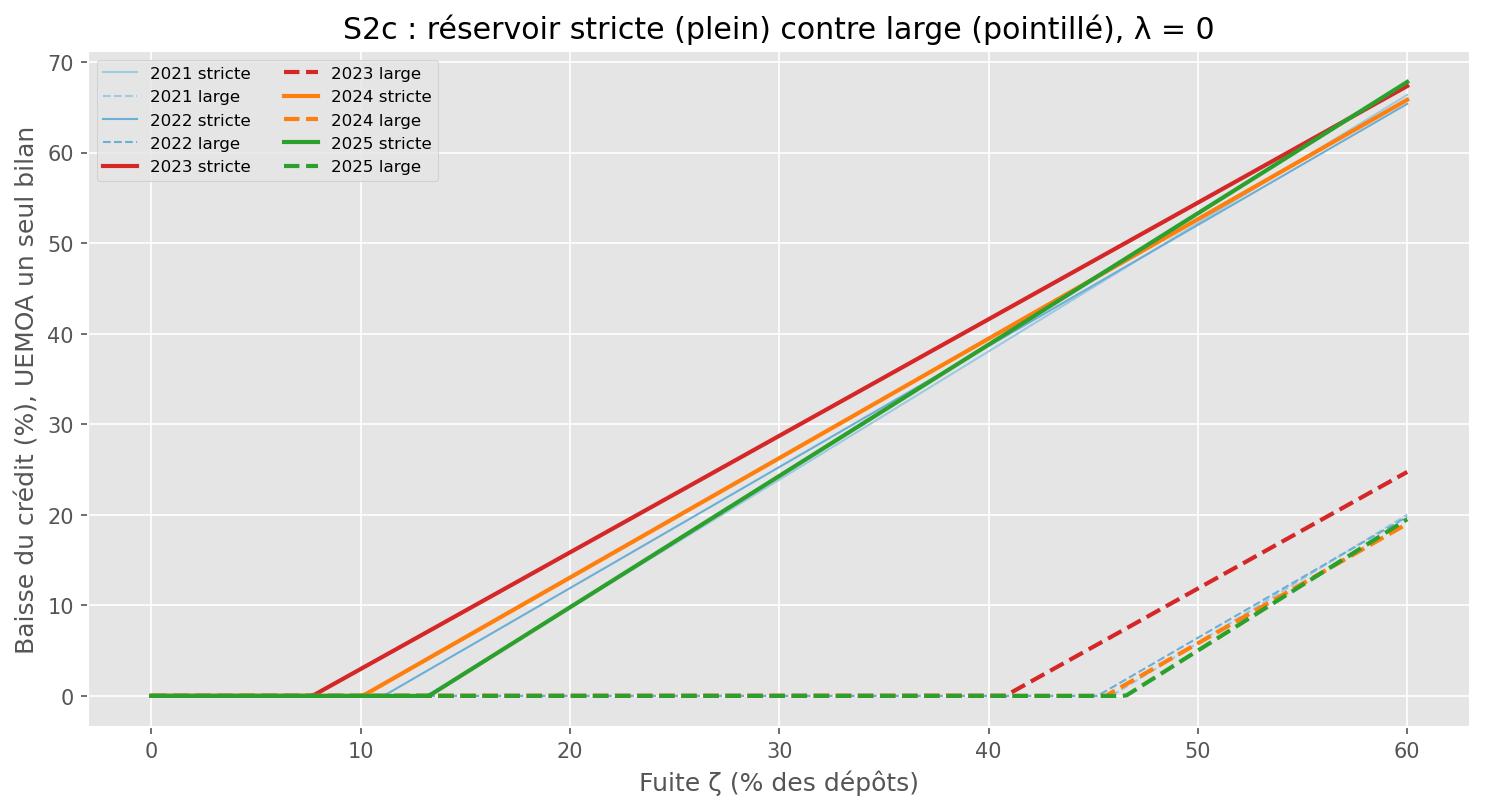
\includegraphics[width=1\textwidth]{S2c_reservoir_stricte_large.png}
		\caption{Matelas stricte (trait plein) contre large (pointillés), jusqu'à 60\,\% de fuite ($\lambda=0$).}
	\end{figure}
	
	\begin{figure}[htbp]
		\centering
		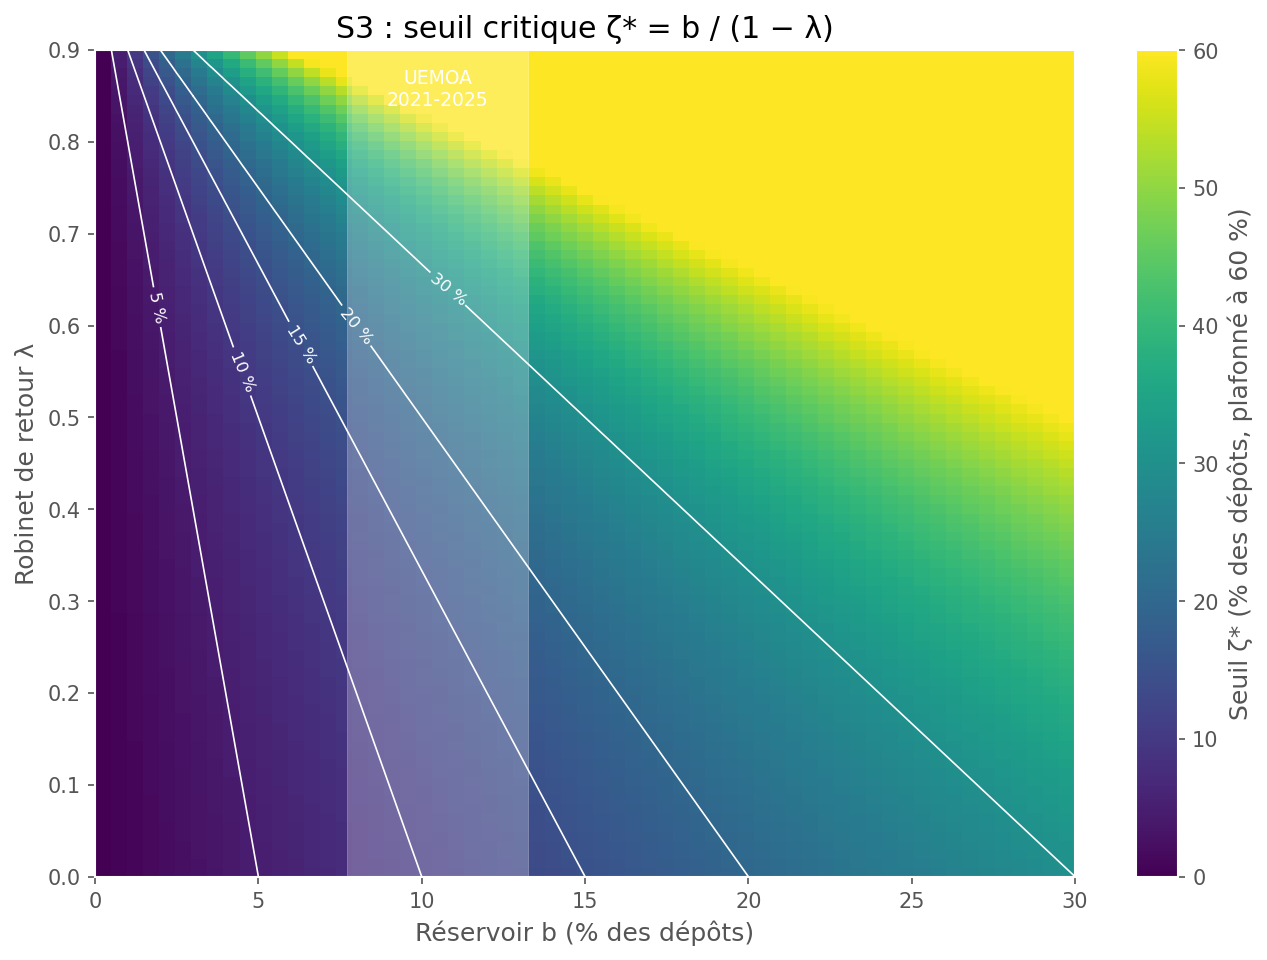
\includegraphics[width=1\textwidth]{S3_carte_sensibilite.png}
		\caption{Seuil critique selon le matelas $b$ et le recyclage $\lambda$.}
	\end{figure}
	
	\begin{figure}[htbp]
		\centering
		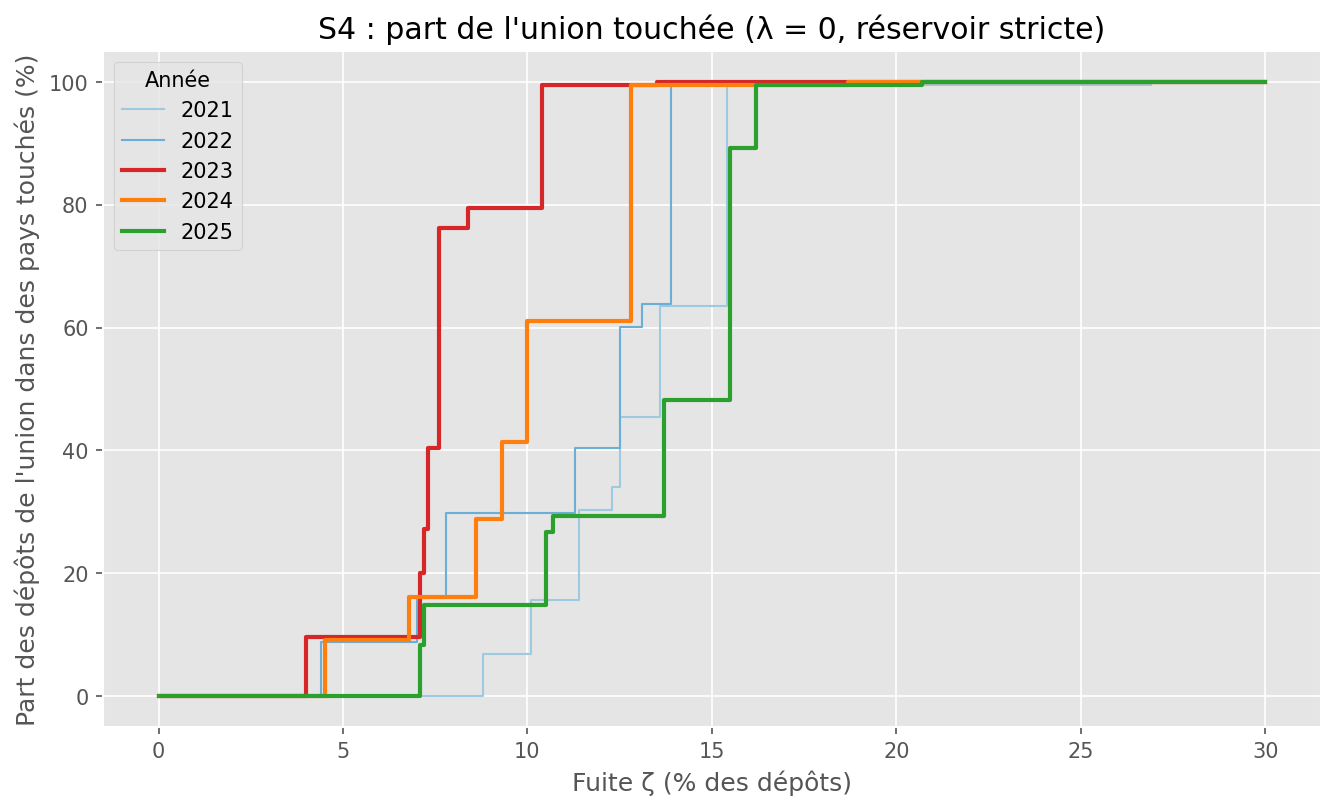
\includegraphics[width=1\textwidth]{S4_part_union_touchee.png}
		\caption{Part des dépôts de l'union située dans des pays au-delà de leur seuil ($\lambda=0$).}
	\end{figure}
	
	\begin{figure}[htbp]
		\centering
		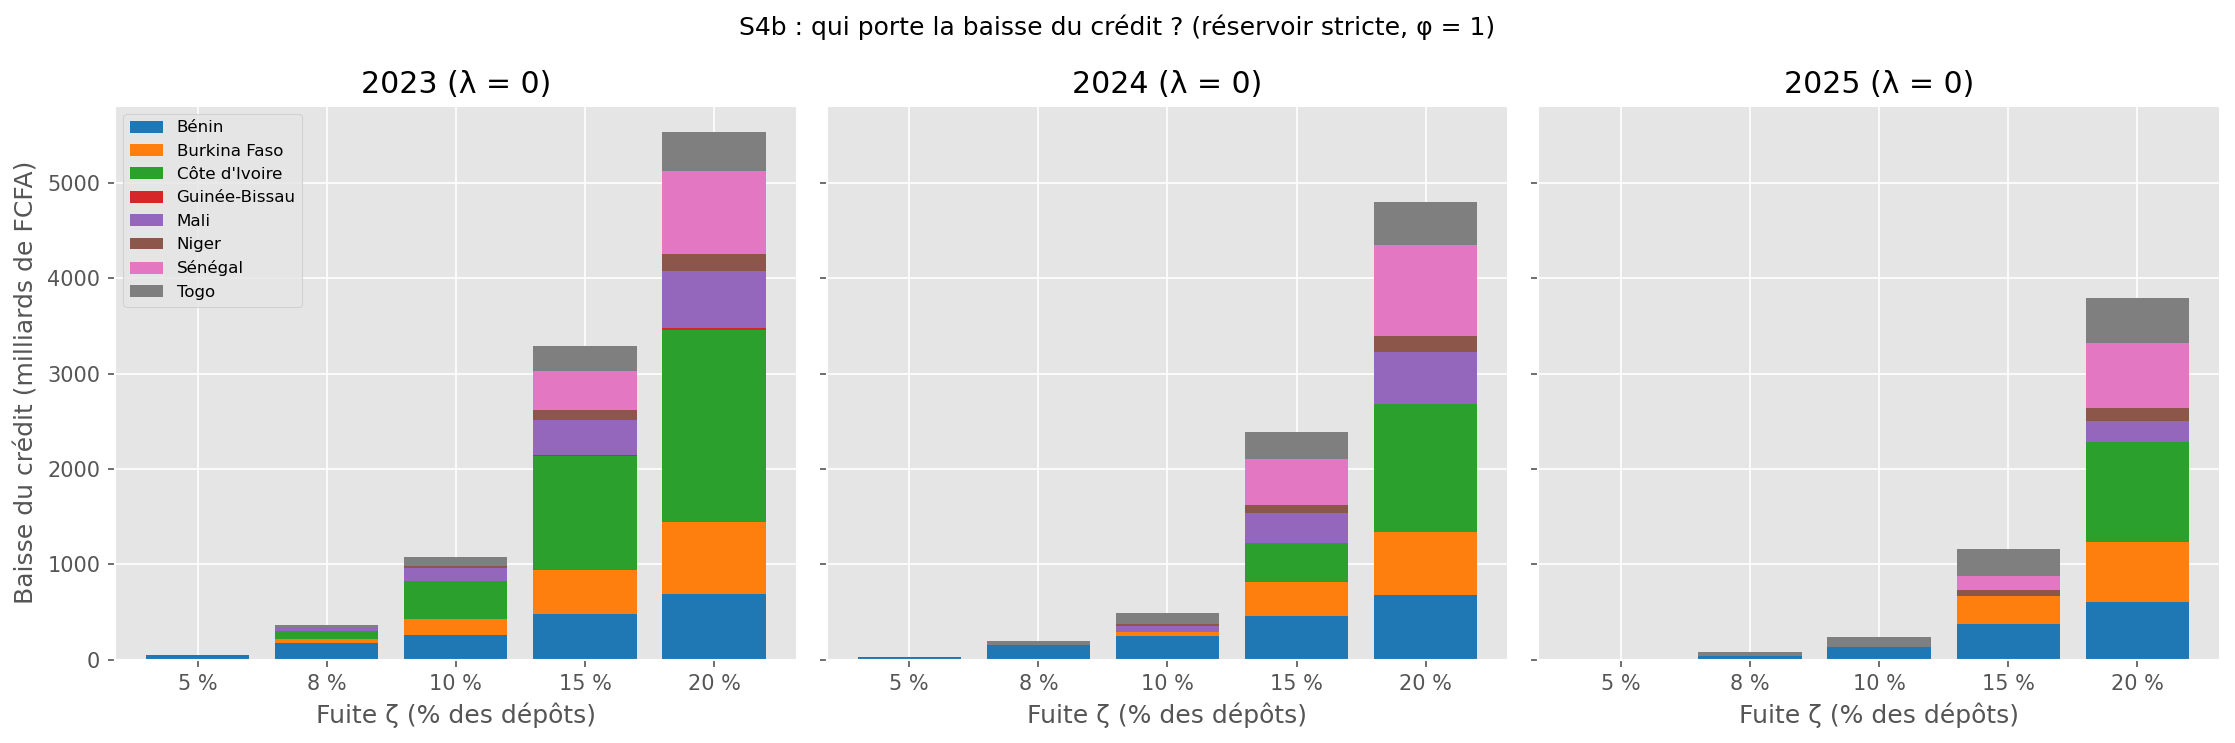
\includegraphics[width=1\textwidth]{S4b_qui_porte_la_baisse.png}
		\caption{Contribution de chaque pays à la baisse du crédit de l'union (milliards de FCFA, $\lambda=0$).}
	\end{figure}
	
	\begin{figure}[htbp]
		\centering
		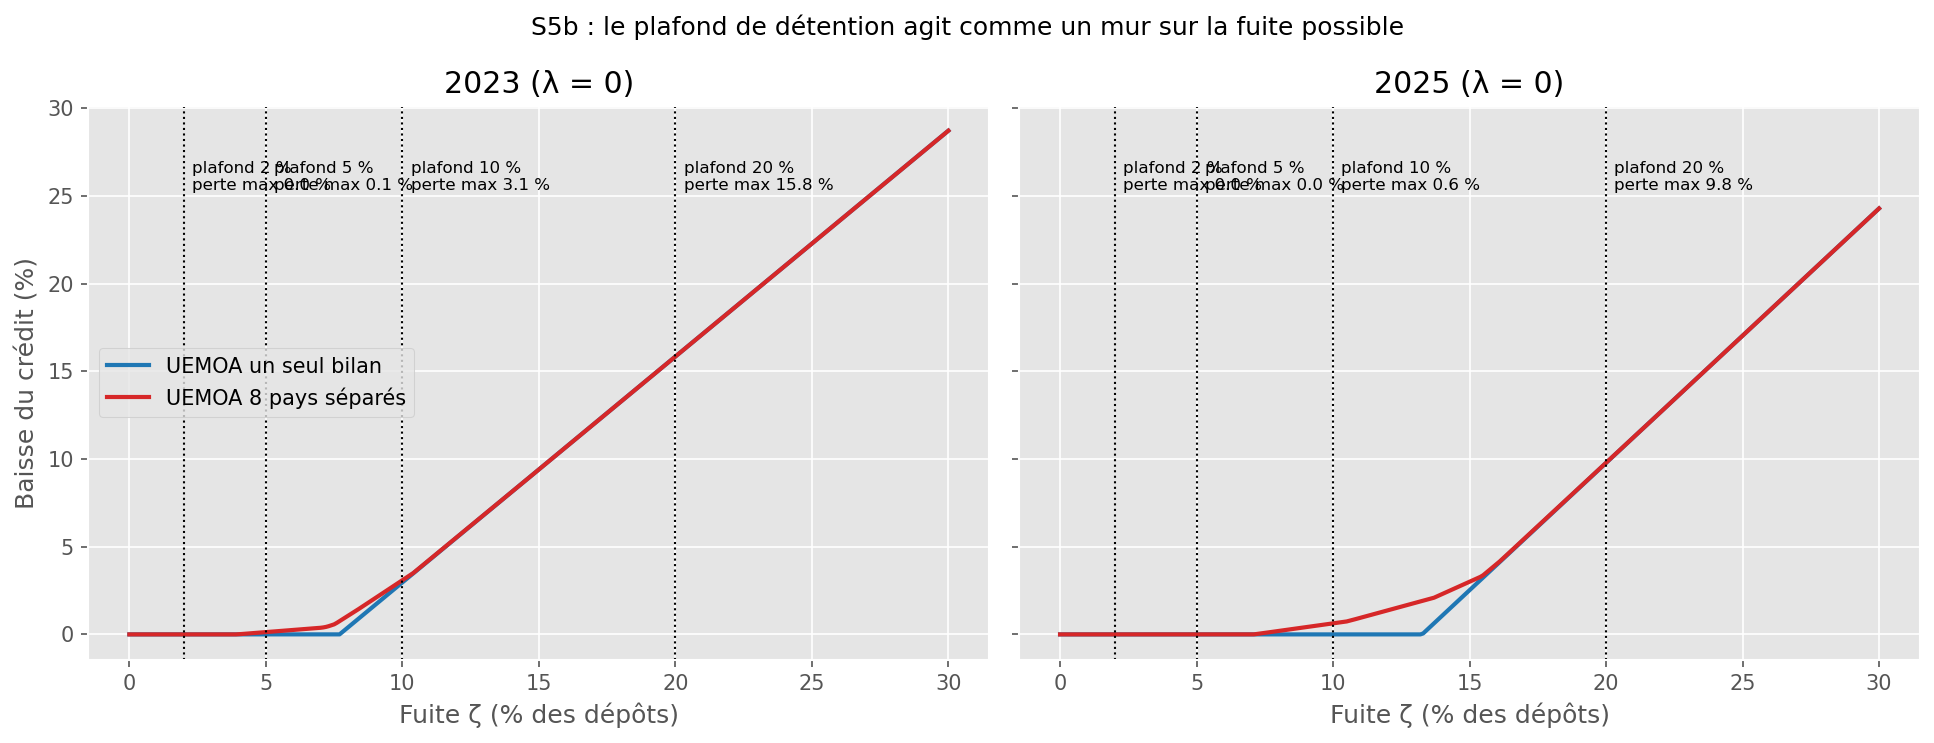
\includegraphics[width=1\textwidth]{S5b_plafond_sur_courbe.png}
		\caption{Plafonds de détention posés sur les courbes de baisse du crédit.}
	\end{figure}
	
	\begin{figure}[htbp]
		\centering
		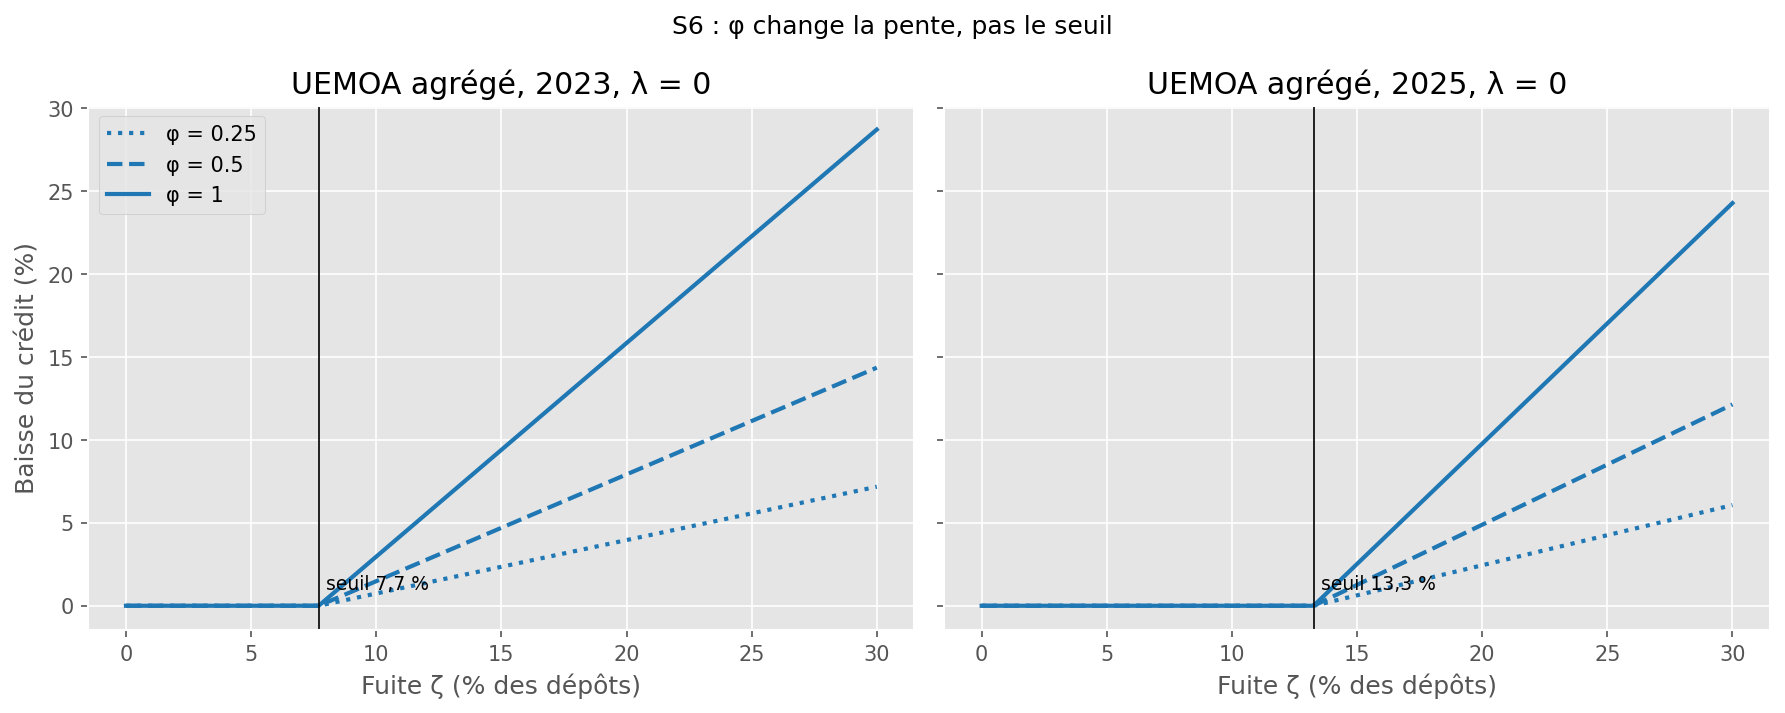
\includegraphics[width=0.9\textwidth]{S6_robustesse_phi.png}
		\caption{Robustesse à $\varphi$ : la pente change, pas le seuil.}
	\end{figure}
	
	\begin{figure}[htbp]
		\centering
		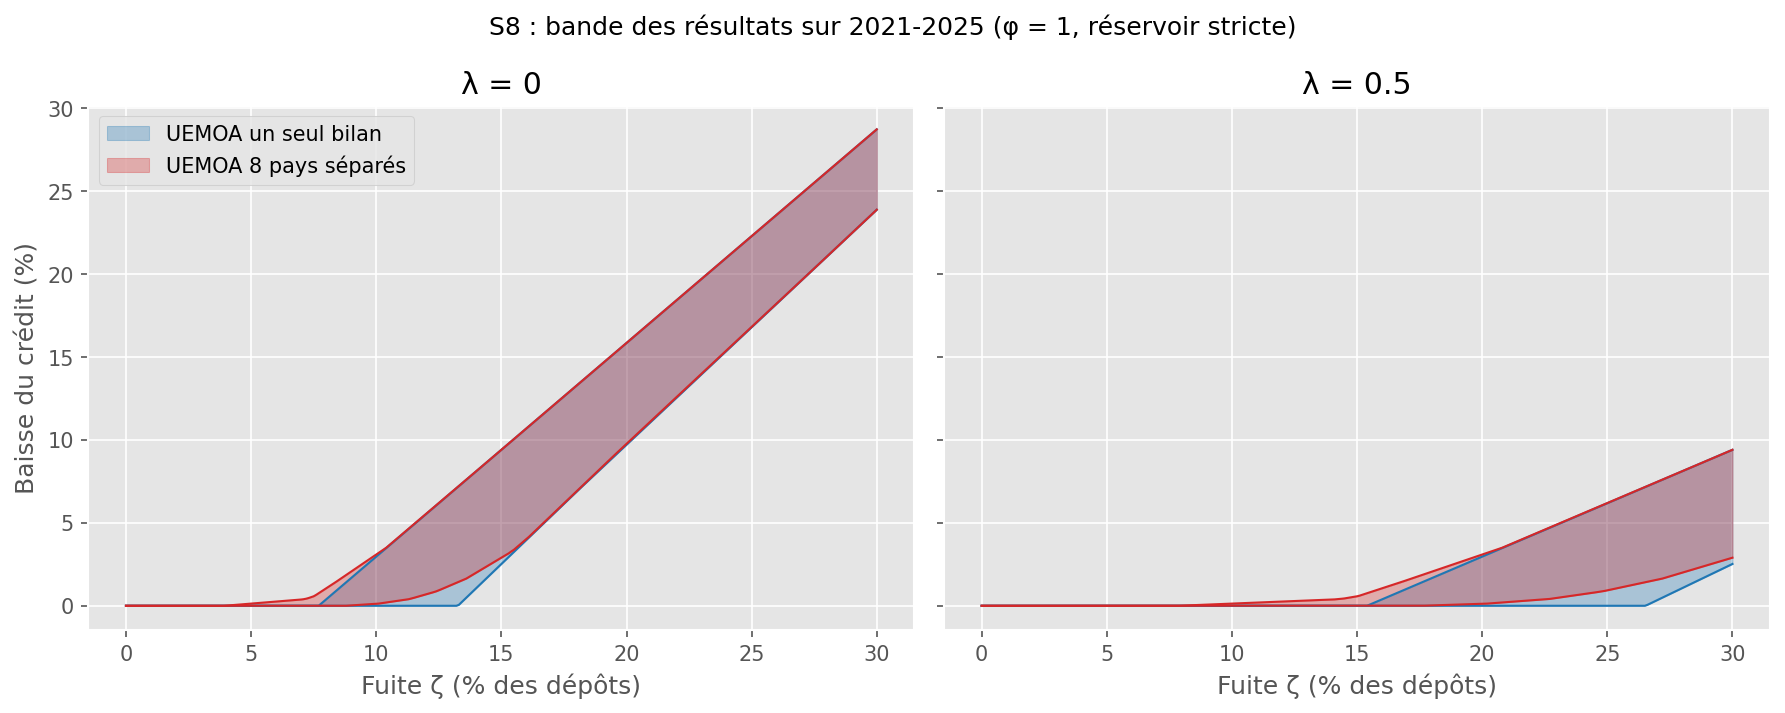
\includegraphics[width=0.9\textwidth]{S8_fourchette.png}
		\caption{Bande min--max des courbes sur 2021--2025.}
	\end{figure}
	
	\begin{figure}[htbp]
		\centering
		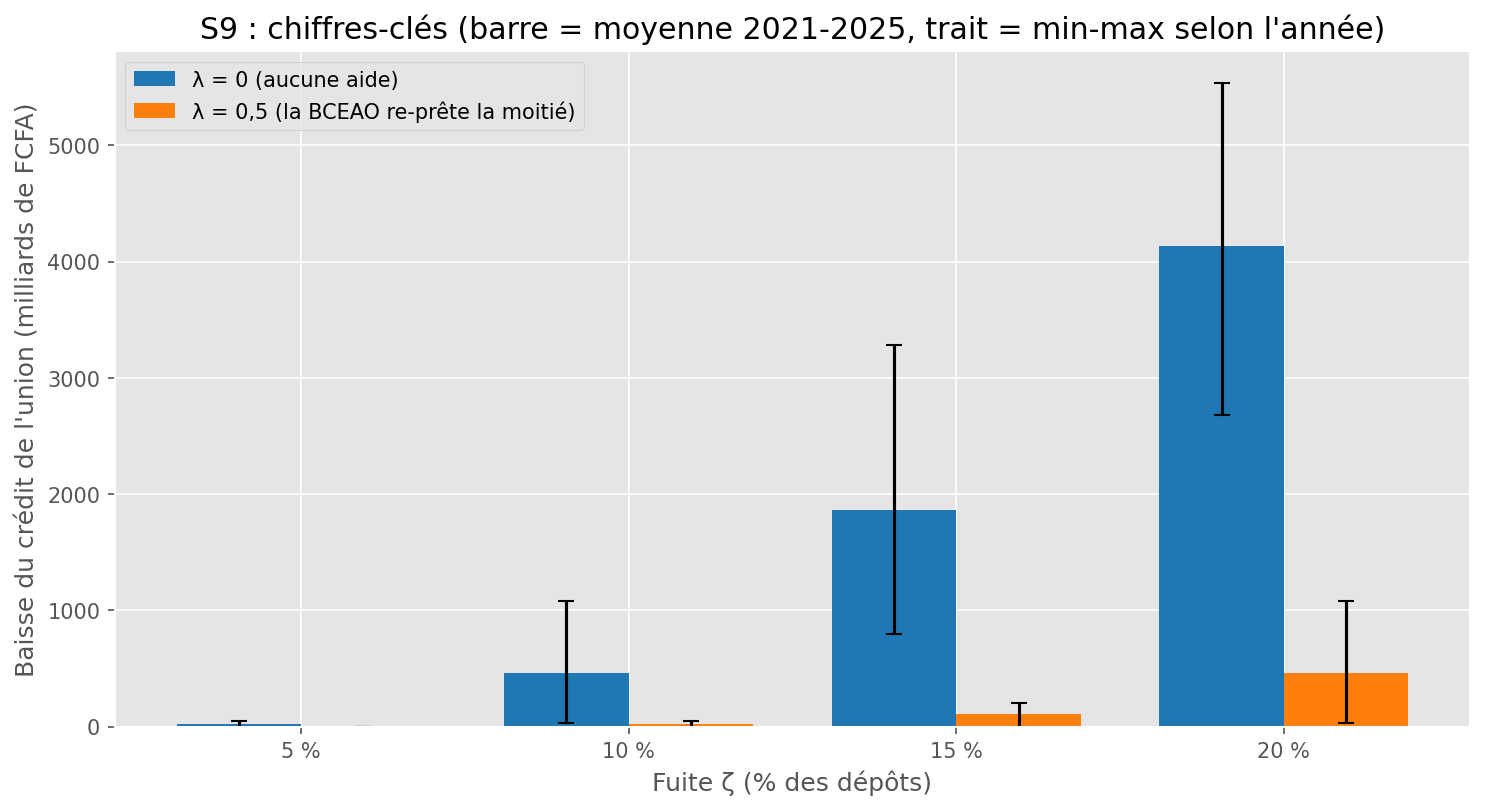
\includegraphics[width=1\textwidth]{S9_chiffres_cles.png}
		\caption{Baisse du crédit de l'union selon la fuite, avec et sans recyclage (moyenne et fourchette 2021--2025).}
	\end{figure}
	
	\begin{figure}[htbp]
		\centering
		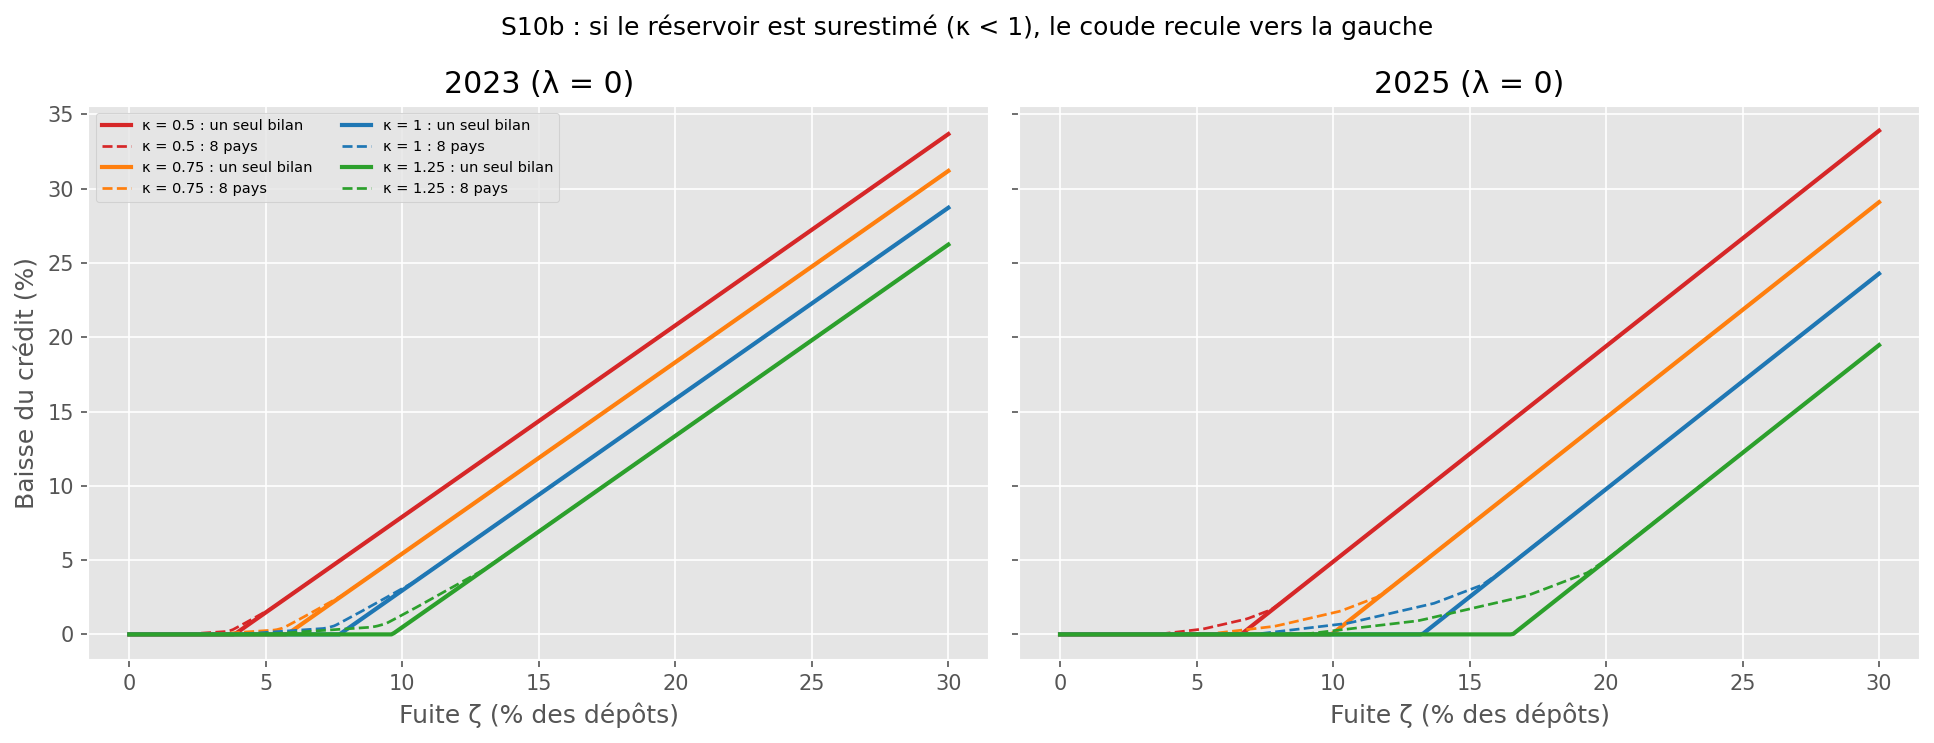
\includegraphics[width=1\textwidth]{S10b_courbes_selon_kappa.png}
		\caption{Courbes de baisse du crédit selon l'erreur de mesure du matelas.}
	\end{figure}
	
	\begin{figure}[htbp]
		\centering
		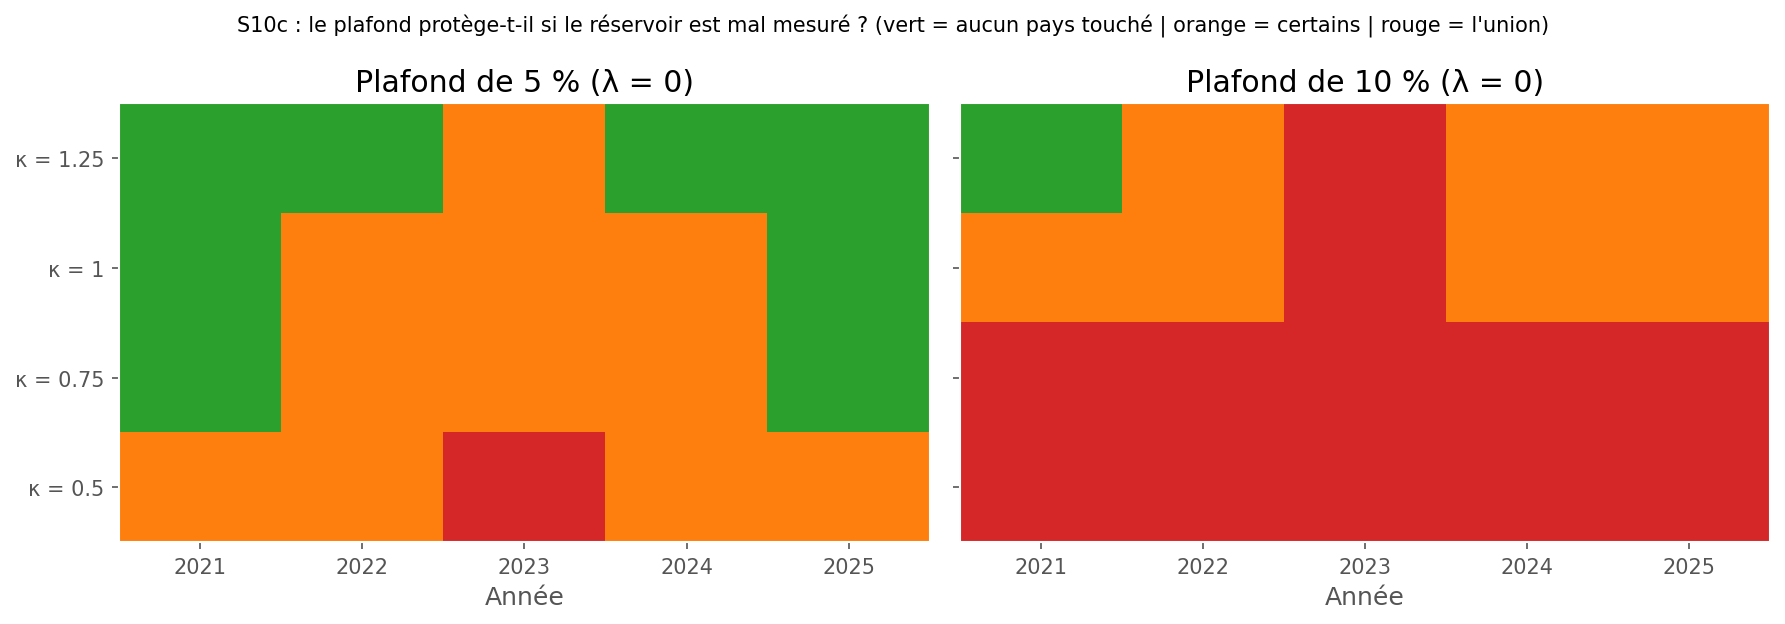
\includegraphics[width=1\textwidth]{S10c_plafond_selon_kappa.png}
		\caption{Résistance des plafonds de 5\,\% et 10\,\% à l'erreur de mesure du matelas.}
	\end{figure}
	
	% =============================================================================
	\section{Reproductibilité et tests de sécurité}\label{app:code}
	% =============================================================================
	
	Les résultats sont produits par le script Python \texttt{simulation\_choc\_retrait.py} à partir du classeur \texttt{Données Extrait.xlsx} (onglet \texttt{Données\_pays}). Le script s'arrête avec un message d'erreur si l'un des onze tests suivants échoue :
	\begin{enumerate}[nosep,label=G\arabic*.]
		\item l'exemple chiffré (100 de dépôts, 80 de prêts, fuite de 10\,\%, matelas de 6\,\%) donne exactement une baisse de 5\,\% ;
		\item pour $\lambda=1$, aucune baisse nulle part ;
		\item la baisse ne diminue jamais quand la fuite augmente ;
		\item sous le seuil critique, la baisse est nulle (tous pays, toutes années) ;
		\item l'agrégat ne dépasse jamais la somme des pays (inégalité de Jensen) ;
		\item les poids des huit pays totalisent 100\,\% chaque année ;
		\item toute baisse est comprise entre 0 et 100\,\%, sans valeur manquante ;
		\item le matelas de l'union égale celui calculé indépendamment dans le classeur de données ;
		\item $\kappa=1$ redonne exactement le cas de base ;
		\item le seuil est proportionnel à $\kappa$ ;
		\item tous les graphiques annoncés existent.
	\end{enumerate}
	
	% =============================================================================
	\begin{thebibliography}{99}
		\setlength{\itemsep}{2pt}
		
		\bibitem[Adalid et al.(2022)]{adalid2022}
		Adalid, R., Álvarez-Blázquez, Á., Assenmacher, K., Burlon, L., Dimou, M., López-Quiles, C., Martín Fuentes, N., Meller, B., Muñoz, M.~A., Radulova, P., Rodriguez d'Acri, C., Shakir, T., Šílová, G., Soons, O., Ventula Veghazy, A. (2022).
		\newblock Central bank digital currency and bank intermediation: Exploring different approaches for assessing the effects of a digital euro on euro area banks.
		\newblock \emph{ECB Occasional Paper Series}, n°~293, mai 2022.
		
		\bibitem[Ahnert et al.(2023)]{ahnert2023}
		Ahnert, T., Hoffmann, P., Leonello, A., Porcellacchia, D. (2023).
		\newblock Central bank digital currency and financial stability.
		\newblock \emph{ECB Working Paper Series}, n°~2783.
		
		\bibitem[Andolfatto(2021)]{andolfatto2021}
		Andolfatto, D. (2021).
		\newblock Assessing the impact of central bank digital currency on private banks.
		\newblock \emph{Economic Journal}, 131(634), 525--540.
		
		\bibitem[Bidder et al.(2024)]{bidder2024}
		Bidder, R., Jackson, T., Rottner, M. (2024).
		\newblock CBDC and banks: Disintermediating fast and slow.
		\newblock \emph{Deutsche Bundesbank Discussion Paper}, n°~15/2024 (version : BIS Working Paper n°~1280, 2025).
		
		\bibitem[Bindseil(2020)]{bindseil2020}
		Bindseil, U. (2020).
		\newblock Tiered CBDC and the financial system.
		\newblock \emph{ECB Working Paper Series}, n°~2351.
		
		\bibitem[Bouis et al.(2024)]{bouis2024}
		Bouis, R., Gelos, G., Miettinen, P., Nakamura, F., Nier, E., Soderberg, G. (2024).
		\newblock Central bank digital currencies and financial stability: Balance sheet analysis and policy choices.
		\newblock \emph{IMF Working Paper}, WP/24/226.
		
		\bibitem[Brunnermeier et Niepelt(2019)]{brunnermeier2019}
		Brunnermeier, M.~K., Niepelt, D. (2019).
		\newblock On the equivalence of private and public money.
		\newblock \emph{Journal of Monetary Economics}, 106, 27--41.
		
		\bibitem[Burlon et al.(2024)]{burlon2024}
		Burlon, L., Muñoz, M.~A., Smets, F. (2024).
		\newblock The optimal quantity of CBDC in a bank-based economy.
		\newblock \emph{American Economic Journal: Macroeconomics}, 16(4), 172--217.
		
		\bibitem[Chiu et al.(2023)]{chiu2023}
		Chiu, J., Davoodalhosseini, S.~M., Jiang, J., Zhu, Y. (2023).
		\newblock Bank market power and central bank digital currency: Theory and quantitative assessment.
		\newblock \emph{Journal of Political Economy}, 131(5), 1213--1248.
		
		\bibitem[Di Maggio et al.(2024)]{dimaggio2024}
		Di Maggio, M. et al. (2024).
		\newblock Impact of retail CBDC on digital payments and bank deposits: Evidence from India.
		\newblock \emph{NBER Working Paper}, n°~32457.
		
		\bibitem[Diamond et Dybvig(1983)]{diamond1983}
		Diamond, D.~W., Dybvig, P.~H. (1983).
		\newblock Bank runs, deposit insurance, and liquidity.
		\newblock \emph{Journal of Political Economy}, 91(3), 401--419.
		
		\bibitem[Fritz et al.(2024)]{fritz2024}
		Fritz, B., Krüger, U., Wong, L.~H. (2024).
		\newblock Digital euro: Short-term effects on the liquidity of German banks considering holding limits.
		\newblock \emph{Deutsche Bundesbank Technical Paper}, n°~05/2024.
		
		\bibitem[Keister et Sanches(2023)]{keister2023}
		Keister, T., Sanches, D. (2023).
		\newblock Should central banks issue digital currency?
		\newblock \emph{Review of Economic Studies}, 90(1), 404--431.
		
		\bibitem[Kumhof et Noone(2018)]{kumhof2018}
		Kumhof, M., Noone, C. (2018).
		\newblock Central bank digital currencies --- design principles and balance sheet implications.
		\newblock \emph{Bank of England Staff Working Paper}, n°~725 ; version publiée dans \emph{Economic Analysis and Policy}, 71 (2021), 553--572.
		
		\bibitem[Meller et Soons(2023)]{meller2023}
		Meller, B., Soons, O. (2023).
		\newblock Know your (holding) limits: CBDC, financial stability and central bank reliance.
		\newblock \emph{ECB Occasional Paper Series}, n°~326 (version : DNB Working Paper n°~771).
		
		\bibitem[Ree(2023)]{ree2023}
		Ree, J. (2023).
		\newblock Nigeria's eNaira, one year after.
		\newblock \emph{IMF Working Paper}, WP/23/104.
		
		\bibitem[Saxegaard(2006)]{saxegaard2006}
		Saxegaard, M. (2006).
		\newblock Excess liquidity and effectiveness of monetary policy: Evidence from Sub-Saharan Africa.
		\newblock \emph{IMF Working Paper}, WP/06/115.
		
		\bibitem[Schilling et al.(2024)]{schilling2024}
		Schilling, L., Fernández-Villaverde, J., Uhlig, H. (2024).
		\newblock Central bank digital currency: When price and bank stability collide.
		\newblock \emph{Journal of Monetary Economics}.
		
		\bibitem[Sun et Rizaldy(2023)]{sun2023}
		Sun, Rizaldy (2023).
		\newblock Some Lessons from Asian E-Money Schemes for the Adoption of Central Bank Digital Currency 
		\emph{IMF Working Paper}, WP/23/123 
		
		\bibitem[Tadenyo(2021)]{tadenyo2021}
		Tadenyo, Y.~D. (2021).
		\newblock Liquidité bancaire et financement de l'économie dans l'UEMOA.
		\newblock \emph{COFEB, Document d'Étude et de Recherche}, n°~COFEB/DER/2021/04, décembre 2021.
		
		\bibitem[Trinnou(2023)]{trinnou2023}
		Trinnou, G.~M. (2023).
		\newblock Impact du mobile money sur l'efficacité de la politique monétaire : cas de l'UEMOA.
		\newblock \emph{COFEB, Document d'Étude et de Recherche}, n°~COFEB/DER/2023/03, décembre 2023.
		
		\bibitem[Whited et al.(2023)]{whited2023}
		Whited, T.~M., Wu, Y., Xiao, K. (2023).
		\newblock Will central bank digital currency disintermediate banks 
		\newblock \emph{IHS Working Paper}, n°~47 
		
		\bigskip
		\noindent\textbf{Sources de données.}
		Commission Bancaire de l'UMOA, \emph{Rapports annuels}, exercices 2021, 2023, 2024 et 2025 ; Banque Centrale des États de l'Afrique de l'Ouest (BCEAO).
		
	\end{thebibliography}
	
\end{document}